% How the Robot Sees -- perception, predicates and the grounding-evaluation branch
% Build: tectonic -X compile perception_guide.tex   (figures/ holds the plots and frames)
\documentclass[11pt,a4paper]{article}

\usepackage[margin=2.1cm,headheight=14pt]{geometry}
\usepackage{lmodern}
\usepackage[T1]{fontenc}
\usepackage{microtype}
\usepackage{xcolor}
\usepackage{graphicx}
\usepackage{amsmath}
\usepackage{tikz}
\usetikzlibrary{arrows.meta,positioning,shapes.geometric,shapes.misc,fit,backgrounds,calc,shadows,decorations.pathreplacing}
\usepackage[most]{tcolorbox}
\usepackage{listings}
\usepackage{booktabs}
\usepackage{tabularx}
\usepackage{enumitem}
\usepackage{fontawesome5}
\usepackage{fancyhdr}
\usepackage{titlesec}
\usepackage{float}
\usepackage{needspace}
\usepackage{textcomp}
\usepackage[hidelinks]{hyperref}

% ---------------------------------------------------------------- colours (as the v1 guide)
\definecolor{ink}{HTML}{1F2933}
\definecolor{sky}{HTML}{2B6CB0}
\definecolor{skylight}{HTML}{EBF4FF}
\definecolor{leaf}{HTML}{2F855A}
\definecolor{leaflight}{HTML}{E6FFFA}
\definecolor{sun}{HTML}{B7791F}
\definecolor{sunlight}{HTML}{FFFAEB}
\definecolor{rose}{HTML}{C53030}
\definecolor{roselight}{HTML}{FFF5F5}
\definecolor{grape}{HTML}{6B46C1}
\definecolor{grapelight}{HTML}{F3EEFF}
\definecolor{stone}{HTML}{718096}
\definecolor{stonelight}{HTML}{F4F6F8}
\definecolor{codebg}{HTML}{F7F9FB}

\color{ink}
\hypersetup{colorlinks=true,linkcolor=sky,urlcolor=sky}

\titleformat{\section}{\Large\bfseries\color{sky}}{\thesection}{0.8em}{}[{\color{sky!40}\titlerule[1pt]}]
\titleformat{\subsection}{\large\bfseries\color{ink}}{\thesubsection}{0.7em}{}
\pagestyle{fancy}
\fancyhf{}
\fancyhead[L]{\small\color{stone}\faEye\ \ How the Robot Sees}
\fancyhead[R]{\small\color{stone}perception/grounding-evaluation}
\fancyfoot[C]{\small\color{stone}\thepage}
\renewcommand{\headrulewidth}{0.4pt}
\setlist{itemsep=2pt,topsep=4pt}
\newcommand{\sectionbreak}{\needspace{24\baselineskip}}
\newcommand{\subsectionbreak}{\needspace{18\baselineskip}}

\newtcolorbox{eli5}{enhanced,colback=sunlight,colframe=sun,boxrule=0.8pt,arc=3mm,
  title={\faChild\ \ In plain words},fonttitle=\bfseries,coltitle=white}
\newtcolorbox{changeit}{enhanced,before upper={\raggedright},colback=leaflight,colframe=leaf,boxrule=0.8pt,arc=3mm,
  title={\faWrench\ \ Where it lives in the code},fonttitle=\bfseries}
\newtcolorbox{careful}{enhanced,before upper={\raggedright},colback=roselight,colframe=rose,boxrule=0.8pt,arc=3mm,
  title={\faExclamationTriangle\ \ Careful},fonttitle=\bfseries}
\newtcolorbox{keyidea}{enhanced,before upper={\raggedright},colback=skylight,colframe=sky,boxrule=0.8pt,arc=3mm,
  title={\faLightbulb\ \ Key idea},fonttitle=\bfseries}
\newtcolorbox{cmd}[1][]{enhanced,breakable,colback=ink!92,colframe=ink,coltext=white,boxrule=0pt,
  arc=2mm,left=6pt,right=6pt,top=4pt,bottom=4pt,fontupper=\ttfamily\small,#1}

\lstdefinestyle{py}{language=Python,basicstyle=\ttfamily\footnotesize,backgroundcolor=\color{codebg},
  keywordstyle=\color{grape}\bfseries,commentstyle=\color{leaf}\itshape,stringstyle=\color{sun!80!black},
  numbers=none,frame=l,framerule=2pt,rulecolor=\color{sky},
  breaklines=true,columns=fullflexible,keepspaces=true,showstringspaces=false,xleftmargin=8pt,
  aboveskip=6pt,belowskip=6pt,upquote=true}
\lstset{style=py}
\newcommand{\code}[1]{\texttt{\detokenize{#1}}}
\newcommand{\srcref}[1]{{\small\color{stone}\faCode\ \texttt{\detokenize{#1}}}}

\tikzset{
  >={Stealth[length=2.6mm]},
  box/.style={draw=#1,fill=#1!8,rounded corners=3pt,thick,align=center,inner sep=6pt,font=\small},
  box/.default=sky,
  pill/.style={draw=#1,fill=#1!12,rounded rectangle,thick,align=center,inner sep=5pt,font=\small},
  pill/.default=sky,
  flow/.style={->,thick,draw=ink!70},
  dflow/.style={->,thick,dashed,draw=ink!55},
  lbl/.style={font=\scriptsize,text=ink!80,align=center},
  zone/.style={draw=#1,fill=#1!4,rounded corners=6pt,thick,dashed,inner sep=10pt},
}

\begin{document}

% ================================================================ TITLE
\begin{titlepage}
\centering
\vspace*{1.2cm}
{\color{sky}\fontsize{30}{36}\selectfont\bfseries How the Robot Sees\par}
\vspace{0.4cm}
{\Large\color{stone} Predicates, providers, planners --- and what the\\[2pt]
\code{perception/grounding-evaluation} branch changes\par}
\vspace{1.2cm}
\begin{tikzpicture}[scale=0.95]
  \node[box=grape,minimum width=3cm,minimum height=1.4cm] (eyes) at (0,0) {\faEye\\[2pt]\textbf{Eyes}\\\scriptsize perception provider};
  \node[box=sky,minimum width=3cm,minimum height=1.4cm] (reg) at (4.2,0) {\faList\\[2pt]\textbf{Facts}\\\scriptsize predicates};
  \node[box=sun,minimum width=3cm,minimum height=1.4cm] (brain) at (8.4,0) {\faBrain\\[2pt]\textbf{Brain}\\\scriptsize planner};
  \node[box=leaf,minimum width=3cm,minimum height=1.4cm] (hands) at (8.4,-2.6) {\faHandPaper\\[2pt]\textbf{Hands}\\\scriptsize skills};
  \node[box=stone,minimum width=3cm,minimum height=1.4cm] (world) at (0,-2.6) {\faCube\\[2pt]\textbf{World}\\\scriptsize simulator};
  \draw[flow] (eyes) -- node[lbl,above]{true / false / ?} (reg);
  \draw[flow] (reg) -- node[lbl,above]{read} (brain);
  \draw[flow] (brain) -- node[lbl,right]{one skill} (hands);
  \draw[flow] (hands) -- node[lbl,above]{actions} (world);
  \draw[flow] (world) -- node[lbl,left]{RGB-D images} (eyes);
\end{tikzpicture}
\vfill
\begin{keyidea}
The robot never reads the simulator's answer key. It has to \emph{see} the mug in
camera images, turn what it sees into a few true/false/unknown \textbf{facts}
(predicates), and let a \textbf{planner} choose the next \textbf{skill} from those
facts. This branch measures how good those facts are and makes them better ---
without ever letting a wrong ``true'' through.
\end{keyidea}
\vspace{0.5cm}
{\color{stone}Olusola --- perception and object grounding\par}
\end{titlepage}

\tableofcontents
\newpage

% ================================================================ 1
\section{The big picture: eyes, facts, brain, hands}

A run of the hanging-mug task is a loop. Each \emph{turn}, the robot looks, decides
one thing to do, does it, and looks again.

\begin{center}
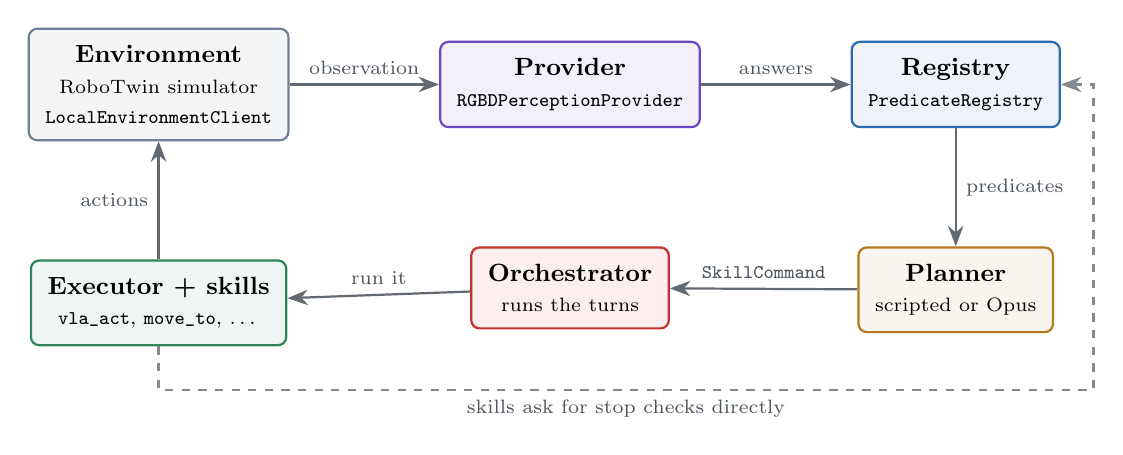
\begin{tikzpicture}[node distance=1.5cm and 1.9cm]
  \node[box=stone] (env) {\textbf{Environment}\\\scriptsize RoboTwin simulator\\\scriptsize\code{LocalEnvironmentClient}};
  \node[box=grape,right=of env] (prov) {\textbf{Provider}\\\scriptsize\code{RGBDPerceptionProvider}};
  \node[box=sky,right=of prov] (reg) {\textbf{Registry}\\\scriptsize\code{PredicateRegistry}};
  \node[box=sun,below=1.5cm of reg] (plan) {\textbf{Planner}\\\scriptsize scripted or Opus};
  \node[box=leaf,below=1.5cm of env] (skill) {\textbf{Executor + skills}\\\scriptsize\code{vla_act}, \code{move_to}, \dots};
  \node[box=rose,below=1.5cm of prov] (orch) {\textbf{Orchestrator}\\\scriptsize runs the turns};
  \draw[flow] (env) -- node[lbl,above]{observation} (prov);
  \draw[flow] (prov) -- node[lbl,above]{answers} (reg);
  \draw[flow] (reg) -- node[lbl,right]{predicates} (plan);
  \draw[flow] (plan) -- node[lbl,above]{\code{SkillCommand}} (orch);
  \draw[flow] (orch) -- node[lbl,above]{run it} (skill);
  \draw[flow] (skill) -- node[lbl,left]{actions} (env);
  \draw[dflow] (skill.south) -- ++(0,-0.55) -| node[lbl,below,pos=0.25]{skills ask for stop checks directly} ($(plan.east)+(0.5,0)$) |- (reg.east);
\end{tikzpicture}
\end{center}

\begin{eli5}
Think of a person tidying a kitchen with their eyes half closed. Their \textbf{eyes}
(the provider) report short facts: ``the mug is in my hand'', ``the mug is standing on
the table''. Their \textbf{brain} (the planner) only hears those facts and picks the next
move. Their \textbf{hands} (skills) carry out the move, and stop early if a fact says
``done'' or ``not safe''. If the eyes say ``I'm not sure'', a careful person waits
instead of guessing.
\end{eli5}

\begin{center}
\small
\begin{tabularx}{\textwidth}{@{}lXl@{}}
\toprule
\textbf{Piece} & \textbf{Its one job} & \textbf{File} \\
\midrule
Environment & Run the simulator, return RGB-D images & \code{harness/environment/local.py} \\
Provider & Turn images into facts & \code{harness/perception/grounding.py} \\
Registry & One place to ask for any fact & \code{harness/predicates/registry.py} \\
Planner & Choose the next skill & \code{harness/planner/} \\
Skills & Move the robot, with safety stops & \code{harness/skills/} \\
Orchestrator & Run turn after turn until done & \code{harness/runtime/orchestrator.py} \\
\bottomrule
\end{tabularx}
\end{center}

% ================================================================ 2
\section{Predicates: the facts the robot believes}

A \textbf{predicate} is a named yes/no question about the scene, such as
``is the mug lifted?''. Every answer is a \code{PredicateResult}:

\begin{lstlisting}
PredicateResult(name="release_ready", value=True | False | None,
                source="perception", observation_sequence=432,
                reason="mug_silhouette_meets_local_table")
\end{lstlisting}

The \code{reason} is a short searchable string saying \emph{why}. It is how we debug a
wrong answer. The full list of names is \code{PREDICATE_NAMES} in
\code{harness/predicates/registry.py}.

\subsection{Three answers, not two}

\begin{center}
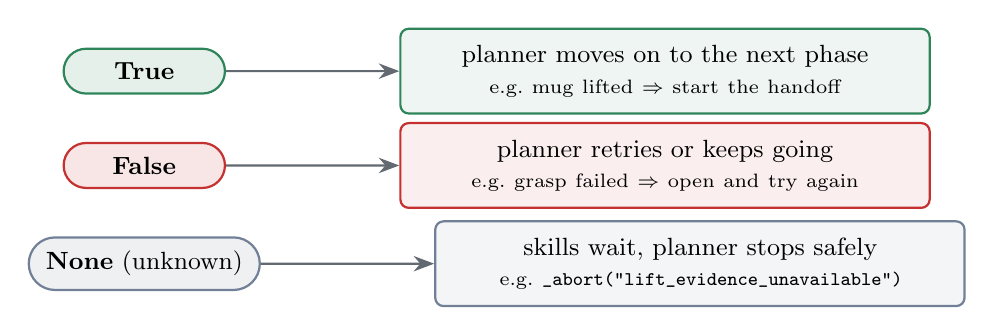
\begin{tikzpicture}[node distance=0.6cm]
  \node[pill=leaf,minimum width=2.4cm] (t) {\textbf{True}};
  \node[pill=rose,minimum width=2.4cm,below=of t] (f) {\textbf{False}};
  \node[pill=stone,minimum width=2.4cm,below=of f] (u) {\textbf{None} (unknown)};
  \node[box=leaf,right=2.2cm of t,text width=6.3cm] (ta) {planner moves on to the next phase\\\scriptsize e.g.\ mug lifted $\Rightarrow$ start the handoff};
  \node[box=rose,right=2.2cm of f,text width=6.3cm] (fa) {planner retries or keeps going\\\scriptsize e.g.\ grasp failed $\Rightarrow$ open and try again};
  \node[box=stone,right=2.2cm of u,text width=6.3cm] (ua) {skills wait, planner stops safely\\\scriptsize e.g.\ \code{_abort("lift_evidence_unavailable")}};
  \draw[flow] (t) -- (ta); \draw[flow] (f) -- (fa); \draw[flow] (u) -- (ua);
\end{tikzpicture}
\end{center}

\begin{careful}
A wrong \textbf{true} is the dangerous mistake. A wrong \code{release_ready = true}
makes the robot open its gripper while the mug is lying on its side --- or in mid air.
A wrong \textbf{unknown} only costs time. That is why every fix in this branch
prefers ``unknown'' to a guess, and why we always report \textbf{precision}
(``when it says true, is it true?'') alongside recall.
\end{careful}

\subsection{The perception predicates this branch measures}

\begin{center}
\small
\begin{tabularx}{\textwidth}{@{}lXcl@{}}
\toprule
\textbf{Predicate} & \textbf{True when} & \textbf{Latches} & \textbf{Unlocks} \\
\midrule
\code{mug_lifted} & the mug has been lifted at some point & yes & HANDOFF \\
\code{release_ready} & the mug is upright and touching the table \emph{now} & no & opening the gripper \\
\code{mug_staged_on_table} & \code{release_ready} after an earlier lift & no & the right-arm grasp \\
\code{right_mug_lifted} & the right gripper alone has held the mug up & yes & HANG \\
\bottomrule
\end{tabularx}
\end{center}

\textbf{Latching} means ``once true, stays true''. A milestone such as ``the mug was
lifted'' remains a fact even if the mug is dropped later, and the planner keeps the
phase it unlocked.

\subsection{Where predicates are used, from start to end of a run}

\begin{center}
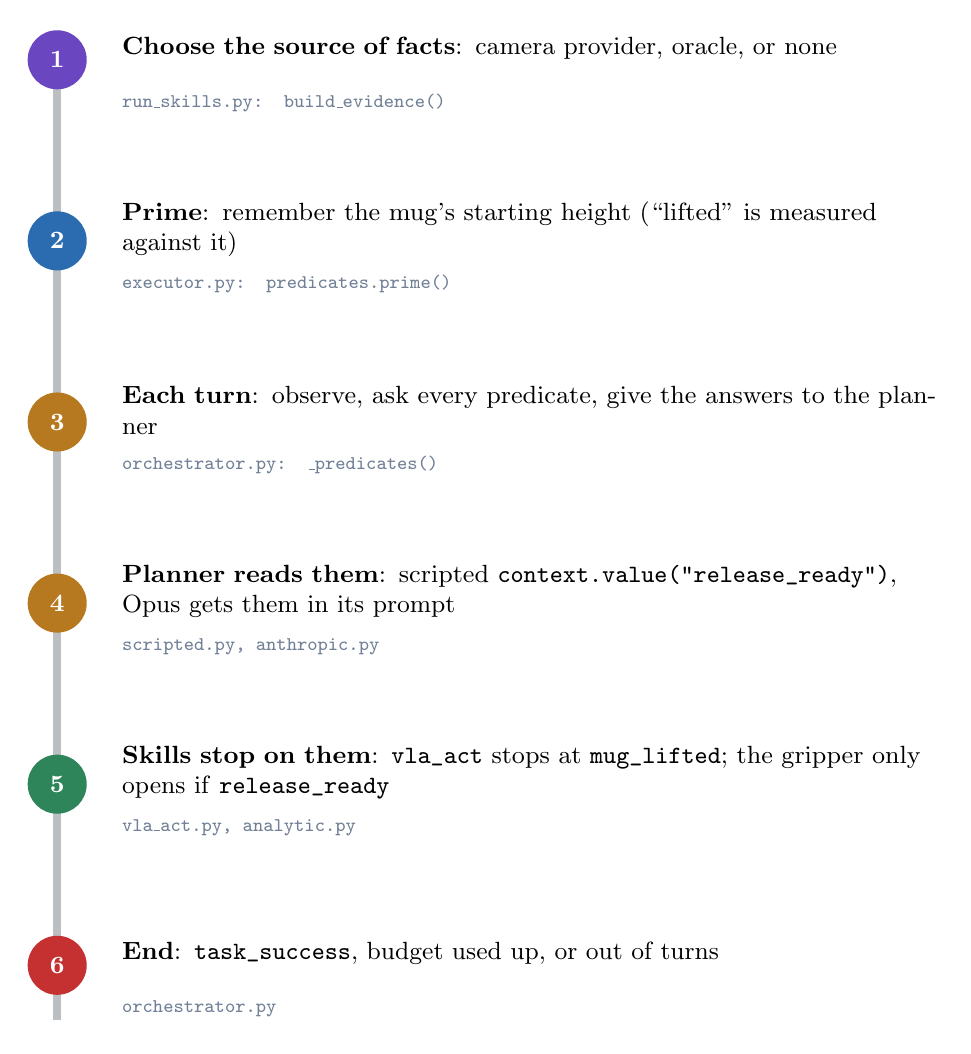
\begin{tikzpicture}[x=1cm,y=1cm]
  \draw[ink!30,line width=3pt] (0,0) -- (0,-12.2);
  \foreach \y/\n/\col/\t/\f in {
     0/1/grape/{\textbf{Choose the source of facts}: camera provider, oracle, or none}/{run\_skills.py: build\_evidence()},
    -2.3/2/sky/{\textbf{Prime}: remember the mug's starting height (``lifted'' is measured against it)}/{executor.py: predicates.prime()},
    -4.6/3/sun/{\textbf{Each turn}: observe, ask every predicate, give the answers to the planner}/{orchestrator.py: \_predicates()},
    -6.9/4/sun/{\textbf{Planner reads them}: scripted \code{context.value("release_ready")}, Opus gets them in its prompt}/{scripted.py, anthropic.py},
    -9.2/5/leaf/{\textbf{Skills stop on them}: \code{vla_act} stops at \code{mug_lifted}; the gripper only opens if \code{release_ready}}/{vla\_act.py, analytic.py},
    -11.5/6/rose/{\textbf{End}: \code{task_success}, budget used up, or out of turns}/{orchestrator.py}} {
    \node[circle,fill=\col,text=white,font=\bfseries\small,minimum size=0.75cm] at (0,\y) {\n};
    \node[anchor=west,text width=10.3cm,font=\small] at (0.7,\y+0.15) {\t};
    \node[anchor=west,font=\scriptsize\ttfamily,text=stone] at (0.7,\y-0.55) {\f};
  }
\end{tikzpicture}
\end{center}

\begin{keyidea}
Camera predicates are checked at \textbf{turn boundaries} and when a skill checks its
stop condition, not after every single action: SAM 3 is too slow for that.
Answers are cached per observation, so the planner and a skill's stop check can never
see two different answers for the same frame.
\end{keyidea}

% ================================================================ 3
\section{Providers: who answers the questions}

The registry does not work anything out itself. It forwards every question to a
\textbf{provider}:

\begin{lstlisting}
provider = self.perception if self.perception is not None else self.hanging_mug
return provider.evaluate(name, observation, arm=arm)
\end{lstlisting}

Anything with a \code{source} and an \code{evaluate(name, observation, arm)} method is a
provider. That makes providers \textbf{swappable}, like plugs in one socket:

\begin{center}
\begin{tikzpicture}
  \node[box=sky,minimum width=3.2cm,minimum height=1.6cm] (reg) {\textbf{PredicateRegistry}\\\scriptsize same questions\\\scriptsize same answers format};
  \node[box=grape,text width=5.2cm,left=2.2cm of reg,yshift=1.3cm] (cam) {\faCamera\ \textbf{RGBDPerceptionProvider}\\\scriptsize SAM 3 masks + depth $\to$ geometry\\\scriptsize \code{source="perception"} --- real runs};
  \node[box=rose,text width=5.2cm,left=2.2cm of reg,yshift=-1.3cm] (ora) {\faKey\ \textbf{HangingMugPredicates}\\\scriptsize exact simulator poses (oracle)\\\scriptsize \code{source="development_oracle"} --- dev only};
  \node[box=sun,right=1.6cm of reg] (pl) {\textbf{Planner}\\\scriptsize cannot tell\\\scriptsize which is plugged in};
  \draw[flow] (cam) -- (reg); \draw[dflow] (ora) -- (reg); \draw[flow] (reg) -- (pl);
\end{tikzpicture}
\end{center}

\begin{center}
\small
\begin{tabularx}{\textwidth}{@{}lX@{}}
\toprule
\textbf{Run with} & \textbf{What you learn} \\
\midrule
Oracle provider & Does the planner and skill logic work when facts are perfect? \\
Camera provider & Does it still work with real, imperfect perception? \\
No provider & Every answer is \code{None}; skills wait or refuse to act. \\
\bottomrule
\end{tabularx}
\end{center}

\begin{careful}
Name trap: inside \code{HangingMugPredicates}, \code{self.provider} is something else ---
the small function that fetches \code{MugEvidence} (exact positions and contacts) from the
simulator. Same word, one level down. The registry refuses the oracle unless the run
explicitly allows it, so it can never leak into an evaluation.
\end{careful}

There is also a narrow third source, \code{RackSeatReleaseGate}, which answers only
\code{rack_seat_aligned} and is asked first for that one question.

% ================================================================ 4
\section{Planners: the brain}

A planner has exactly one method:

\begin{lstlisting}
def select(self, context: PlannerContext) -> PlannerSelection: ...
\end{lstlisting}

\begin{center}
\begin{tikzpicture}
  \node[box=stone,text width=4.6cm,align=left] (ctx) {\textbf{PlannerContext} (in)\\[2pt]\scriptsize
   \textbullet\ \code{observation}: the images\\
   \textbullet\ \code{predicates}: the facts\\
   \textbullet\ \code{previous}: last skill's result\\
   \textbullet\ \code{remaining_budget}\\
   \textbullet\ memory, visual hints};
  \node[box=sun,right=1.2cm of ctx,minimum height=1.6cm] (sel) {\faBrain\\\textbf{select()}};
  \node[box=leaf,right=1.2cm of sel,text width=5.2cm,align=left] (cmd) {\textbf{SkillCommand} (out)\\[2pt]\scriptsize
   \code{action="vla_act", arm="both",}\\\code{stop="mug_lifted"}\\[3pt]
   \code{action="set_gripper", arm="left",}\\\code{parameters={"value": 1.0}}};
  \draw[flow] (ctx) -- (sel); \draw[flow] (sel) -- (cmd);
\end{tikzpicture}
\end{center}

The \code{stop} field must name a real predicate; this is how a decision by the brain
becomes a safety stop inside the hands.

\begin{center}
\small
\begin{tabularx}{\textwidth}{@{}lXl@{}}
\toprule
\textbf{Planner} & \textbf{How it decides} & \textbf{File} \\
\midrule
\code{GraspRetryPlanner} & fixed script: approach, grasp until lifted, retry if the grasp failed & \code{scripted.py} \\
\code{HandoffPlanner} & scripted full task: left grasp, stage, right grasp, rack, hang & \code{handoff.py} \\
\code{AnthropicPlanner} & Opus sees images + predicates, replies with one checked skill & \code{anthropic.py} \\
\bottomrule
\end{tabularx}
\end{center}

\subsection{The full task as a chain of predicate gates}

\begin{center}
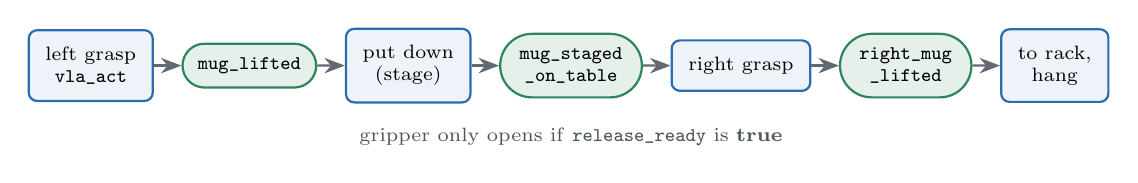
\begin{tikzpicture}[node distance=0.35cm]
  \node[box=sky,font=\scriptsize] (a) {left grasp\\\code{vla_act}};
  \node[pill=leaf,font=\scriptsize,right=of a] (g1) {\code{mug_lifted}};
  \node[box=sky,font=\scriptsize,right=of g1] (b) {put down\\(stage)};
  \node[pill=leaf,font=\scriptsize,right=of b] (g2) {\code{mug_staged}\\\code{_on_table}};
  \node[box=sky,font=\scriptsize,right=of g2] (c) {right grasp};
  \node[pill=leaf,font=\scriptsize,right=of c] (g3) {\code{right_mug}\\\code{_lifted}};
  \node[box=sky,font=\scriptsize,right=of g3] (d) {to rack,\\hang};
  \draw[flow] (a)--(g1); \draw[flow] (g1)--(b); \draw[flow] (b)--(g2); \draw[flow] (g2)--(c); \draw[flow] (c)--(g3); \draw[flow] (g3)--(d);
  \node[lbl,below=0.25cm of g2,text width=6cm] {gripper only opens if \code{release_ready} is \textbf{true}};
\end{tikzpicture}
\end{center}

Each green gate is a predicate the camera provider must answer. If a gate is wrongly
true, the robot skips ahead (for example, lets go of a toppled mug). If it is never
true, the robot stalls. Perception quality \emph{is} task quality.

% ================================================================ 5
\section{How the camera provider actually sees}

\subsection{From pixels to a fact}

\begin{center}
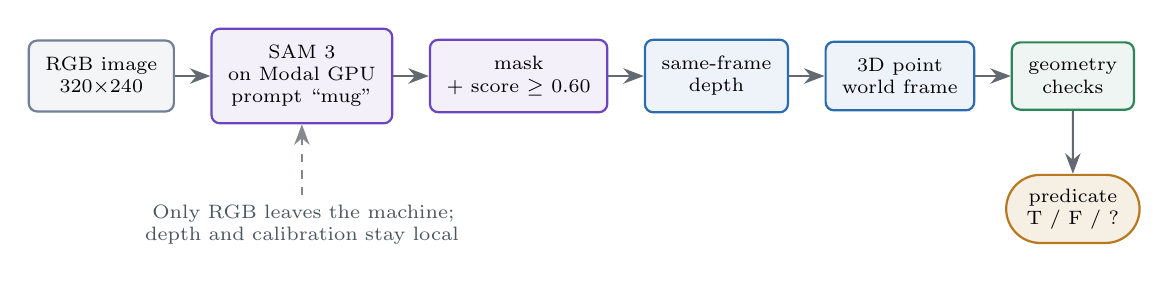
\begin{tikzpicture}[node distance=0.45cm]
  \node[box=stone,font=\scriptsize] (rgb) {RGB image\\\scriptsize 320$\times$240};
  \node[box=grape,font=\scriptsize,right=of rgb] (sam) {SAM 3\\\scriptsize on Modal GPU\\\scriptsize prompt ``mug''};
  \node[box=grape,font=\scriptsize,right=of sam] (mask) {mask\\\scriptsize + score $\ge$ 0.60};
  \node[box=sky,font=\scriptsize,right=of mask] (dep) {same-frame\\depth};
  \node[box=sky,font=\scriptsize,right=of dep] (pt) {3D point\\\scriptsize world frame};
  \node[box=leaf,font=\scriptsize,right=of pt] (geo) {geometry\\checks};
  \node[pill=sun,font=\scriptsize,below=0.8cm of geo] (pred) {predicate\\T / F / ?};
  \draw[flow] (rgb)--(sam); \draw[flow] (sam)--(mask); \draw[flow] (mask)--(dep); \draw[flow] (dep)--(pt); \draw[flow] (pt)--(geo); \draw[flow] (geo)--(pred);
  \node[lbl,below=0.9cm of sam,text width=4.6cm] (n1) {Only RGB leaves the machine;\\depth and calibration stay local};
  \draw[dflow] (n1) -- (sam);
\end{tikzpicture}
\end{center}

\begin{eli5}
SAM 3 is a model that ``colours in'' the pixels belonging to whatever you name. It
paints the mug. The depth image says how far away each pixel is. Combine the two and
you know \emph{where in the room} the mug's visible surface is. Simple geometry then
answers questions like ``is it higher than the table?'' or ``is it touching the table?''.
\end{eli5}

\subsection{Back-projection: one pixel to one 3D point}

\begin{center}
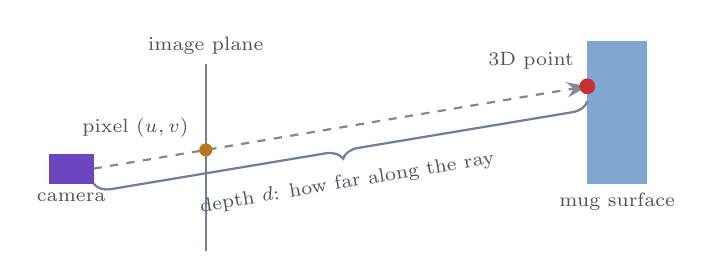
\begin{tikzpicture}[scale=0.95]
  \fill[grape] (0,0) rectangle (0.6,0.4); \node[lbl,below] at (0.3,0) {camera};
  \draw[stone,thick] (2.1,-0.9) -- (2.1,1.6); \node[lbl,above] at (2.1,1.6) {image plane};
  \draw[dflow] (0.6,0.2) -- (7.2,1.3);
  \fill[sun] (2.1,0.45) circle (2.5pt); \node[lbl,anchor=east] at (2.0,0.75) {pixel $(u,v)$};
  \fill[sky!60] (7.2,0.0) rectangle (8.0,1.9); \node[lbl,below] at (7.6,0.0) {mug surface};
  \fill[rose] (7.2,1.3) circle (3pt); \node[lbl,anchor=south east] at (7.15,1.4) {3D point};
  \draw[decorate,decoration={brace,amplitude=6pt,mirror},thick,stone] (0.6,0.0) -- (7.2,1.1)
    node[midway,below=8pt,lbl,sloped] {depth $d$: how far along the ray};
\end{tikzpicture}
\end{center}

\[
\mathbf{X}_{\text{cam}} = d\,K^{-1}\begin{bmatrix}u\\v\\1\end{bmatrix},\qquad
\mathbf{X}_{\text{world}} = R^{\top}\,(\mathbf{X}_{\text{cam}} - \mathbf{t})
\]

$K$ is the lens (intrinsic) matrix; $R,\mathbf{t}$ is the camera's pose
(\code{world_to_camera}, OpenCV convention). In code: \code{(cam - t) @ R}.
The provider takes the \textbf{median} over the mask's pixels so a few bad depth
readings do not move the point.

\begin{careful}
A mug is hollow. Depth at the centre of the opening hits the table \emph{behind} the mug.
That is why a mask is required: the median over the mask's own pixels stays on the mug.
\end{careful}

\subsection{Which camera answers}

\begin{center}
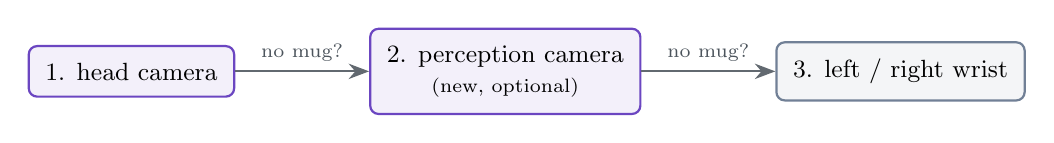
\begin{tikzpicture}[node distance=0.4cm]
  \node[box=grape,font=\small] (h) {1. head camera};
  \node[box=grape,font=\small,right=1.7cm of h] (p) {2. perception camera\\\scriptsize (new, optional)};
  \node[box=stone,font=\small,right=1.7cm of p] (w) {3. left / right wrist};
  \draw[flow] (h) -- node[lbl,above]{no mug?} (p); \draw[flow] (p) -- node[lbl,above]{no mug?} (w);
\end{tikzpicture}
\end{center}

The first camera with a confident, unambiguous mug wins. Wrist cameras move with the
arms and see very close-up, partial views, so they are the last resort.

% ================================================================ 6
\section{What this branch builds: an evaluation loop}

Before this branch we could not say \emph{how often} perception was right. The core of
the branch is a loop that measures it, offline, on saved frames:

\begin{center}
\begin{tikzpicture}[node distance=0.9cm]
  \node[box=rose,text width=3.1cm] (cap) {\faVideo\ \textbf{1. Capture}\\\scriptsize run the policy, save frames every 16 actions + labels};
  \node[box=grape,text width=3.1cm,right=of cap] (cache) {\faCloud\ \textbf{2. SAM 3 cache}\\\scriptsize ask SAM 3 once per frame and camera, save answers};
  \node[box=leaf,text width=3.1cm,right=of cache] (eval) {\faChartBar\ \textbf{3. Evaluate}\\\scriptsize replay through the real provider, compare with labels};
  \node[box=sun,text width=3.1cm,below=1.0cm of eval] (fix) {\faWrench\ \textbf{4. Fix}\\\scriptsize change one rule, with a test};
  \node[box=sky,text width=3.1cm,left=of fix] (probe) {\faSearch\ \textbf{Probe}\\\scriptsize ask SAM 3 new questions on hard frames};
  \draw[flow] (cap) -- (cache); \draw[flow] (cache) -- (eval);
  \draw[flow] ([xshift=-0.5cm]eval.south) -- ([xshift=-0.5cm]fix.north);
  \draw[flow] ([xshift=0.5cm]fix.north) -- node[lbl,right]{re-evaluate\\(CPU, seconds)} ([xshift=0.5cm]eval.south);
  \draw[dflow] (eval) to[bend right=25] (probe); \draw[dflow] (probe) -- (fix);
  \node[pill=rose,font=\scriptsize,above=0.15cm of cap] {GPU (Modal or local)};
  \node[pill=grape,font=\scriptsize,above=0.15cm of cache] {GPU (Modal)};
  \node[pill=leaf,font=\scriptsize,above=0.15cm of eval] {CPU only};
\end{tikzpicture}
\end{center}

\begin{keyidea}
The expensive steps (simulating, running SAM 3) happen \textbf{once}. After that, every
idea for a fix is scored in seconds on CPU, against the same frames, with the runtime's
own code. That turns ``I think this is better'' into ``this is better on 216 frames, and
here are the numbers''.
\end{keyidea}

\subsection{Step 0: the scene viewer}

\code{development/capture/scene_views.py} resets one seed and saves what every camera
sees (RGB, depth, an overview sheet). It never moves the robot. We used it to inspect
camera coverage and to aim the new perception camera.

\subsection{Step 1: labelled capture --- public frames and a private answer key}

\begin{center}
\begin{tikzpicture}
  \node[box=leaf,text width=5.3cm,align=left] (pub) {\faFolderOpen\ \code{observations/} \textbf{(public)}\\[2pt]\scriptsize
  \code{observation_00000416.npz}: RGB + depth + calibration for each camera, joint state.\\Exactly what the robot sees.};
  \node[box=rose,text width=5.3cm,align=left,right=1.6cm of pub] (priv) {\faKey\ \code{labels.jsonl} \textbf{(private)}\\[2pt]\scriptsize
  true mug pose, tilt, contacts, gripper values, and a \textbf{state}: \code{resting}, \code{held_left}, \code{held_right}, \code{staged}, \code{toppled}, \code{off_table}, \dots};
  \draw[rose,line width=2pt] ($(pub.east)!0.5!(priv.west)+(0,1.3)$) -- ($(pub.east)!0.5!(priv.west)+(0,-1.3)$);
  \node[lbl,text=rose] at ($(pub.east)!0.5!(priv.west)+(0,-1.6)$) {wall: labels never reach runtime};
\end{tikzpicture}
\end{center}

The labels are only read by evaluators under \code{development/}. The provider and
planner never see them; that rule is the difference between \emph{measuring}
perception and \emph{cheating}.

\subsection{Step 2: the SAM 3 cache}

SAM 3 runs on a Modal GPU. \code{sam3_cache.py} sends each frame's images once and
stores the raw answers in \code{sam3_cache.json} next to the frames. Later,
\code{CachedSam3Worker} plays them back through the \emph{real} \code{ModalSam3Detector}
client, so camera order and thresholds are exactly the runtime's.

\subsection{Step 3: the evaluator}

\code{perception_evaluation.py} replays every frame through the provider and compares
each predicate answer with the label's truth:

\begin{center}
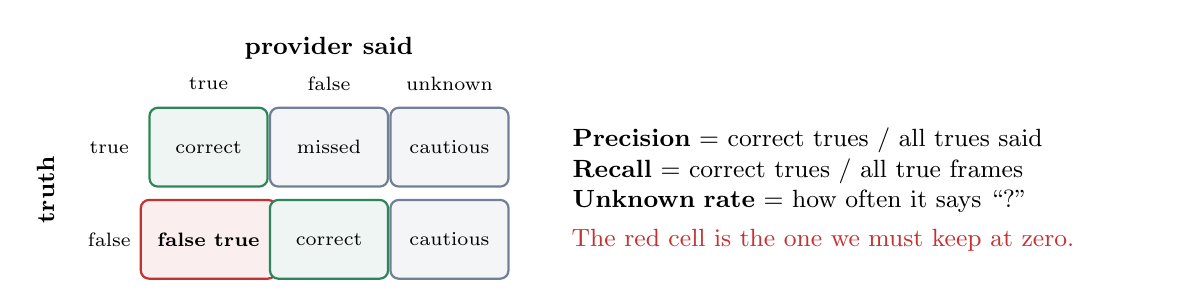
\begin{tikzpicture}[scale=0.9]
  \node[font=\small\bfseries] at (2.7,3.0) {provider said};
  \node[font=\small\bfseries,rotate=90] at (-1.3,1.0) {truth};
  \foreach \x/\t in {1/true,2.7/false,4.4/unknown} \node[font=\scriptsize] at (\x,2.5) {\t};
  \node[font=\scriptsize] at (-0.4,1.6) {true}; \node[font=\scriptsize] at (-0.4,0.3) {false};
  \node[box=leaf,minimum width=1.5cm,minimum height=1cm,font=\scriptsize] at (1,1.6) {correct};
  \node[box=stone,minimum width=1.5cm,minimum height=1cm,font=\scriptsize] at (2.7,1.6) {missed};
  \node[box=stone,minimum width=1.5cm,minimum height=1cm,font=\scriptsize] at (4.4,1.6) {cautious};
  \node[box=rose,minimum width=1.5cm,minimum height=1cm,font=\scriptsize] at (1,0.3) {\textbf{false true}};
  \node[box=leaf,minimum width=1.5cm,minimum height=1cm,font=\scriptsize] at (2.7,0.3) {correct};
  \node[box=stone,minimum width=1.5cm,minimum height=1cm,font=\scriptsize] at (4.4,0.3) {cautious};
  \node[anchor=west,text width=7.2cm,font=\small] at (6,1.0) {
    \textbf{Precision} = correct trues / all trues said\\
    \textbf{Recall} = correct trues / all true frames\\
    \textbf{Unknown rate} = how often it says ``?''\\[3pt]
    \textcolor{rose}{The red cell is the one we must keep at zero.}};
\end{tikzpicture}
\end{center}

\begin{careful}
\textbf{Frames, not seeds, are the unit.} The policy is not deterministic: the same seed
gives a different episode each time. So we compare fixes on the \emph{same saved frames},
never by re-running a seed and hoping it repeats.
\end{careful}

% ================================================================ 7
\section{The fixes, one by one}

\subsection{Fix 1: a perception-only camera}

The head camera looks down from behind the robot; when an arm lifts the mug, the arm
often hides it. We added a fixed RGB-D camera, \code{perception_camera}, on the far side
of the table (\code{harness/environment/perception_cameras.py}). The policy never receives
it and Opus prompts don't use it; it is added after each reset so every seed keeps its
exact scene.

\begin{center}
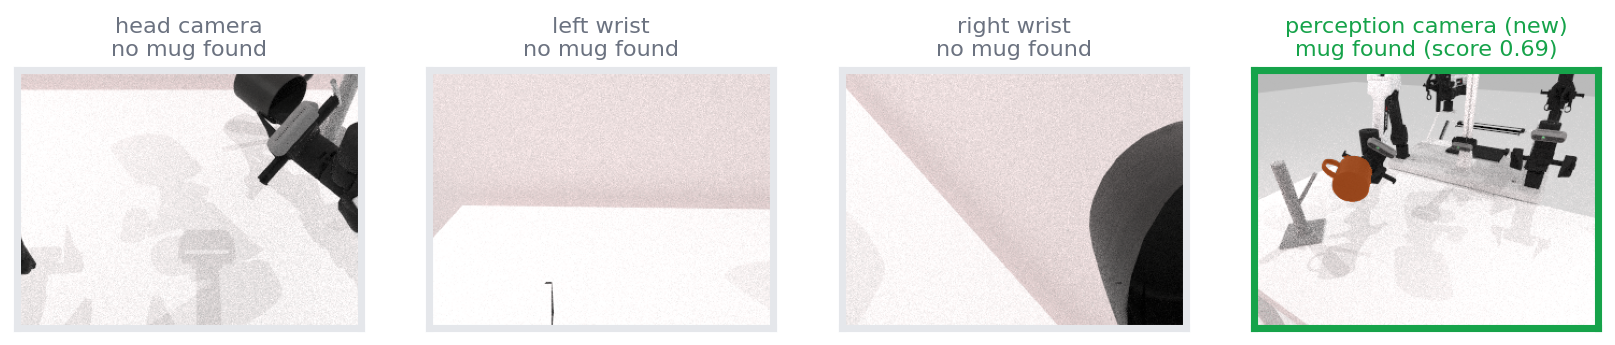
\includegraphics[width=\textwidth]{figures/four_cameras.png}\\
{\small\color{stone}Real frame (seed 0, action 416, mug in the right gripper): SAM 3's
mug mask in orange. Only the new camera finds it.}
\end{center}

\begin{center}
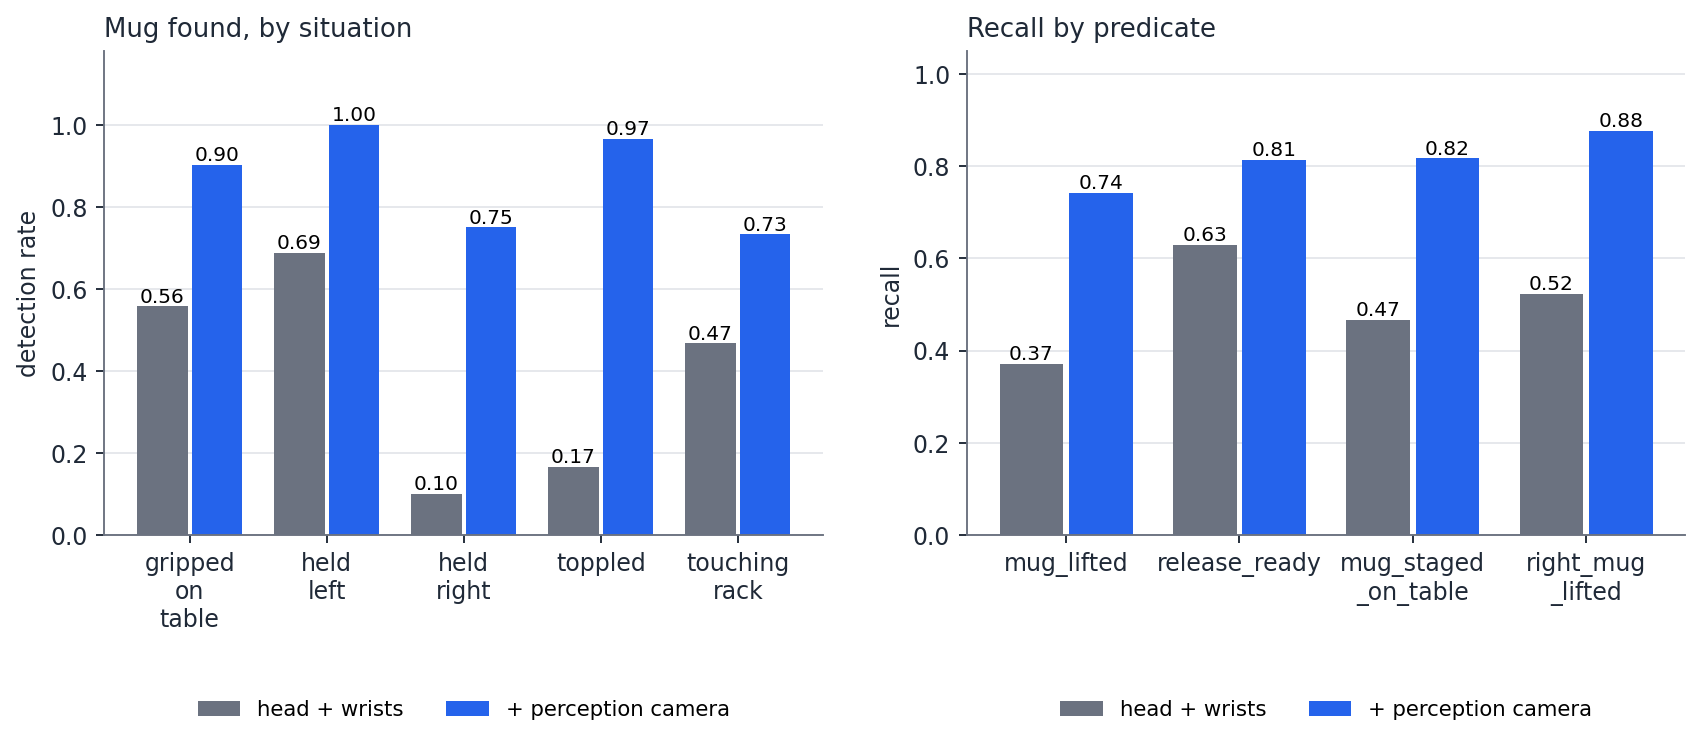
\includegraphics[width=\textwidth]{figures/camera_results.png}\\
{\small\color{stone}Same 216 frames scored with and without the new camera
(\code{--ignore-camera perception_camera}). Precision stays 1.00 in both.}
\end{center}

\subsection{Fix 2: a toppled mug is not ``standing on the table''}

The baseline said \code{release_ready = true} for \textbf{39 of 56} toppled frames: a mug
lying on its side \emph{is} touching the table. Height and shape features overlapped
between upright and toppled mugs. What separates them is \textbf{which way the visible
surface faces}.

\begin{center}
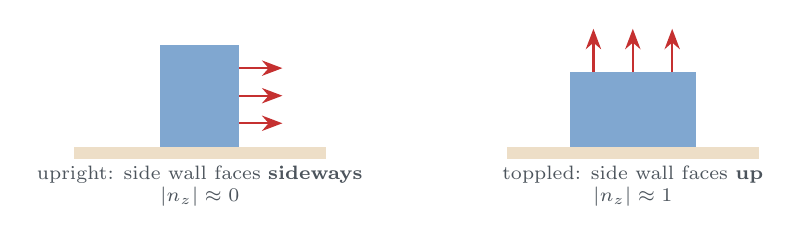
\begin{tikzpicture}
  \begin{scope}
    \fill[sun!25] (-1.6,-0.15) rectangle (1.6,0); \fill[sky!60] (-0.5,0) rectangle (0.5,1.3);
    \foreach \y in {0.3,0.65,1.0} \draw[->,rose,thick] (0.5,\y) -- (1.05,\y);
    \node[lbl] at (0,-0.5) {upright: side wall faces \textbf{sideways}\\$|n_z| \approx 0$};
  \end{scope}
  \begin{scope}[xshift=5.5cm]
    \fill[sun!25] (-1.6,-0.15) rectangle (1.6,0); \fill[sky!60] (-0.8,0) rectangle (0.8,0.95);
    \foreach \x in {-0.5,0,0.5} \draw[->,rose,thick] (\x,0.95) -- (\x,1.5);
    \node[lbl] at (0,-0.5) {toppled: side wall faces \textbf{up}\\$|n_z| \approx 1$};
  \end{scope}
\end{tikzpicture}
\end{center}

For each mask pixel we take the surface normal from neighbouring depth points (a cross
product of the two directions along the surface), rotate it into the world, and keep
$|n_z|$, its vertical part. The median over the mask decides:
$\le 0.25 \Rightarrow$ upright; otherwise \code{mug_surface_faces_up_not_upright}.
Fewer than 300 usable pixels $\Rightarrow$ unknown.

\begin{center}
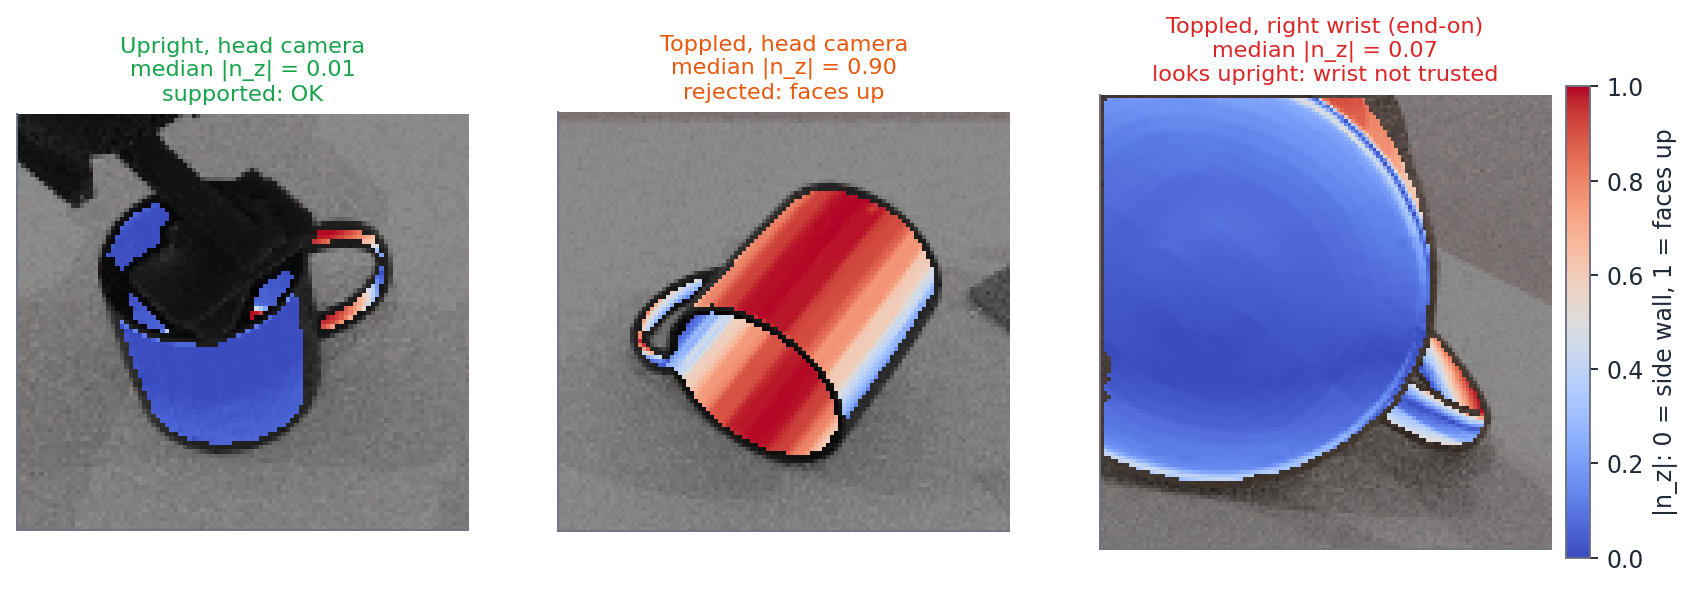
\includegraphics[width=\textwidth]{figures/normals.png}\\
{\small\color{stone}Real masks coloured by $|n_z|$. The third panel is why the rule has a
second part.}
\end{center}

\begin{careful}
\textbf{The fix did not generalise at first.} On new episodes, a wrist camera looking at a
toppled mug \emph{end-on} sees mostly its flat base, which faces sideways --- just like an
upright wall (median 0.04--0.10). So table support is now judged \textbf{only from the head
or perception camera}; a wrist-grounded mug gives
\code{table_support_not_judged_from_wrist_view} (unknown). Every wrist-view
\code{release_ready = true} in all reports had been wrong, so this costs no real recall.
\end{careful}

\begin{center}
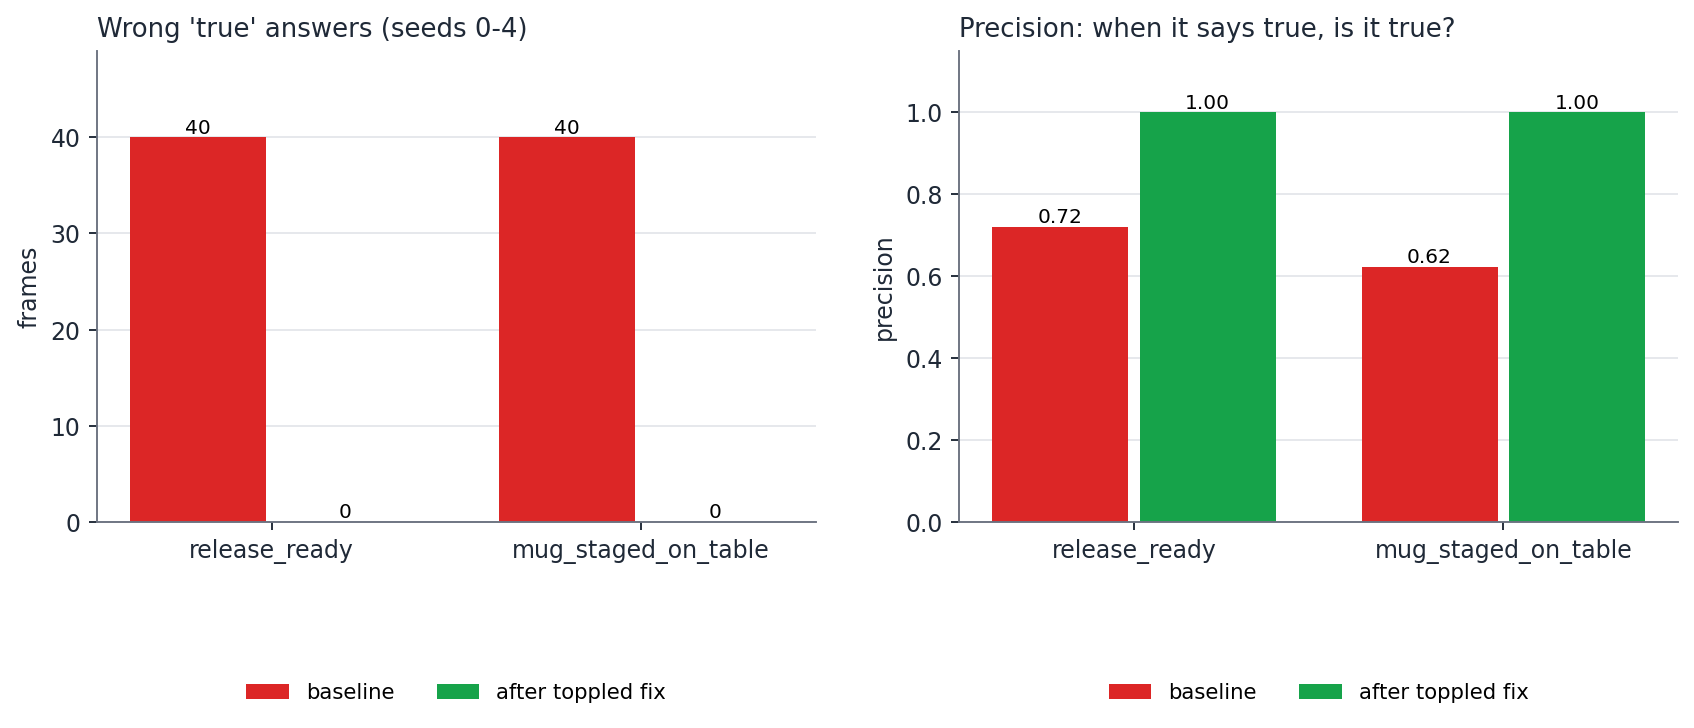
\includegraphics[width=\textwidth]{figures/toppled_results.png}
\end{center}

\begin{careful}
\textbf{Held-out check (seeds 5--9): the head camera can see a toppled mug end-on too.}
In seed 6 the mug fell over with its flat base facing the head camera and lay still for
the rest of the episode. Its visible surface faces sideways (median $|n_z|$ 0.09), exactly
like an upright wall, so table support said ``upright'' in all 26 frames --- 25 wrong
\code{release_ready = true}. Seed 7's toppled mug, side-on to the same camera, was
rejected every time (0.87). The normal test separates \emph{side-on} toppled mugs, not
\emph{end-on} ones, from any camera. Every other held-out frame kept precision 1.00.
\end{careful}

\begin{center}
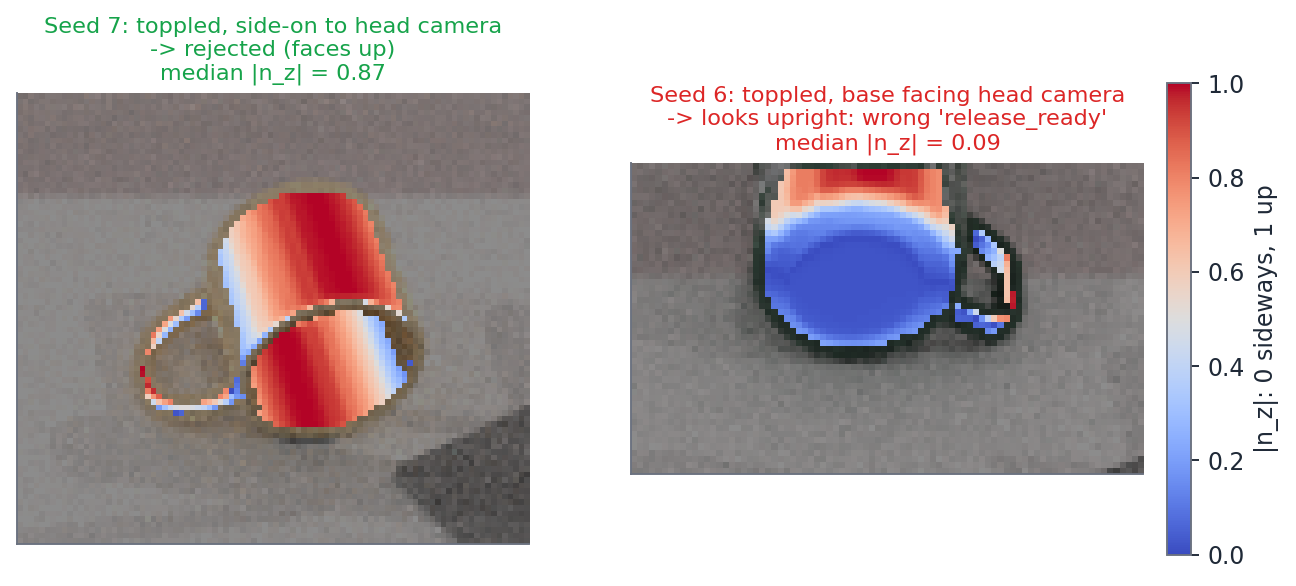
\includegraphics[width=0.8\textwidth]{figures/holdout_end_on.png}\\
{\small\color{stone}Same camera, same rule, frame 640 of two held-out episodes.}
\end{center}

\subsection{Fix 3: wait until the mug stops moving}

\begin{center}
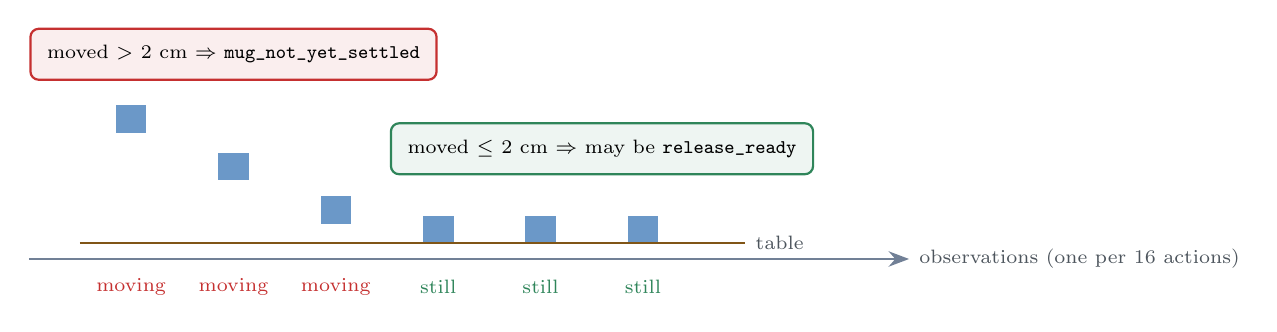
\begin{tikzpicture}[x=1.3cm]
  \draw[->,thick,stone] (0,0) -- (8.6,0) node[right,lbl]{observations (one per 16 actions)};
  \foreach \x/\h/\c in {1/1.6/rose,2/1.0/rose,3/0.45/rose,4/0.2/leaf,5/0.2/leaf,6/0.2/leaf} {
    \fill[sky!70] (\x-0.15,\h) rectangle (\x+0.15,\h+0.35);
    \node[lbl,text=\c] at (\x,-0.35) {\ifnum\x<4 moving\else still\fi};
  }
  \draw[sun!70!black,thick] (0.5,0.2) -- (7,0.2) node[right,lbl]{table};
  \node[box=rose,font=\scriptsize] at (2,2.6) {moved $>$ 2 cm $\Rightarrow$ \code{mug_not_yet_settled}};
  \node[box=leaf,font=\scriptsize] at (5.6,1.4) {moved $\le$ 2 cm $\Rightarrow$ may be \code{release_ready}};
\end{tikzpicture}
\end{center}

A mug being set down can briefly ``meet the table'' in one frame while still moving.
In the captures, mugs being lifted or lowered moved 2.6--4.0 cm between observations,
while 95\% of resting mugs moved less than 2 cm. So table support now needs two
observations in a row that agree within 2 cm (\code{MUG_SETTLED_MAX_STEP_M}).

\subsection{Fix 4: recognising the right-arm lift}

\begin{center}
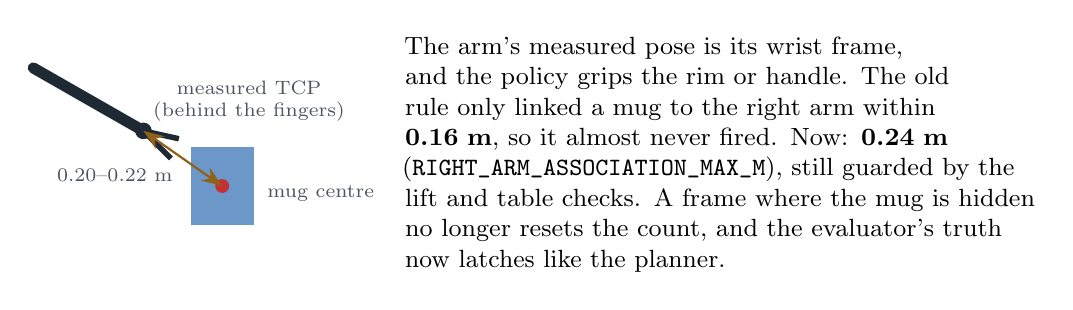
\begin{tikzpicture}
  \draw[ink,line width=4pt,line cap=round] (0,2.4) -- (1.4,1.6);
  \fill[ink] (1.4,1.6) circle (3pt); \node[lbl,above right] at (1.4,1.6) {measured TCP\\(behind the fingers)};
  \draw[ink,line width=2pt] (1.4,1.6) -- (1.75,1.25) (1.4,1.6) -- (1.85,1.5);
  \fill[sky!70] (2.0,0.4) rectangle (2.8,1.4); \fill[rose] (2.4,0.9) circle (2.5pt);
  \node[lbl,right] at (2.85,0.8) {mug centre};
  \draw[<->,thick,sun!80!black] (1.4,1.6) -- (2.4,0.9) node[midway,below left,lbl]{0.20--0.22 m};
  \node[anchor=west,text width=8cm,font=\small] at (4.6,1.3) {
    The arm's measured pose is its wrist frame, and the policy grips the rim or
    handle. The old rule only linked a mug to the right arm within \textbf{0.16 m}, so it
    almost never fired. Now: \textbf{0.24 m} (\code{RIGHT_ARM_ASSOCIATION_MAX_M}),
    still guarded by the lift and table checks. A frame where the mug is hidden no
    longer resets the count, and the evaluator's truth now latches like the planner.};
\end{tikzpicture}
\end{center}

Result: \code{right_mug_lifted} recall 0.09 $\to$ 0.88 with the camera, precision 1.00.

\subsection{Fix 5: a mug on the floor is \texttt{off\_table}, not toppled}

Most remaining ``toppled'' misses were seed 4's mug lying on the \emph{floor}, about
0.70 m below the table and out of every view. That is a labelling problem, not a
perception one. Frames where the mug is 0.20 m or more below its start height are now
labelled \code{off_table}. Toppled detection with the camera: \textbf{28 of 29}.

\subsection{Probe: can a different SAM 3 question find sideways mugs?}

The last real misses (16 frames) are mugs turned on their side in a gripper or at the
rack. The probe asks SAM 3 five prompts (``mug'', ``cup'', ``coffee mug'', ``mug held by
a robot gripper'', ``mug lying on its side'') with scores down to 0.05, and checks each
mask's 3D point against the true mug (hit within 0.10 m).

\begin{center}
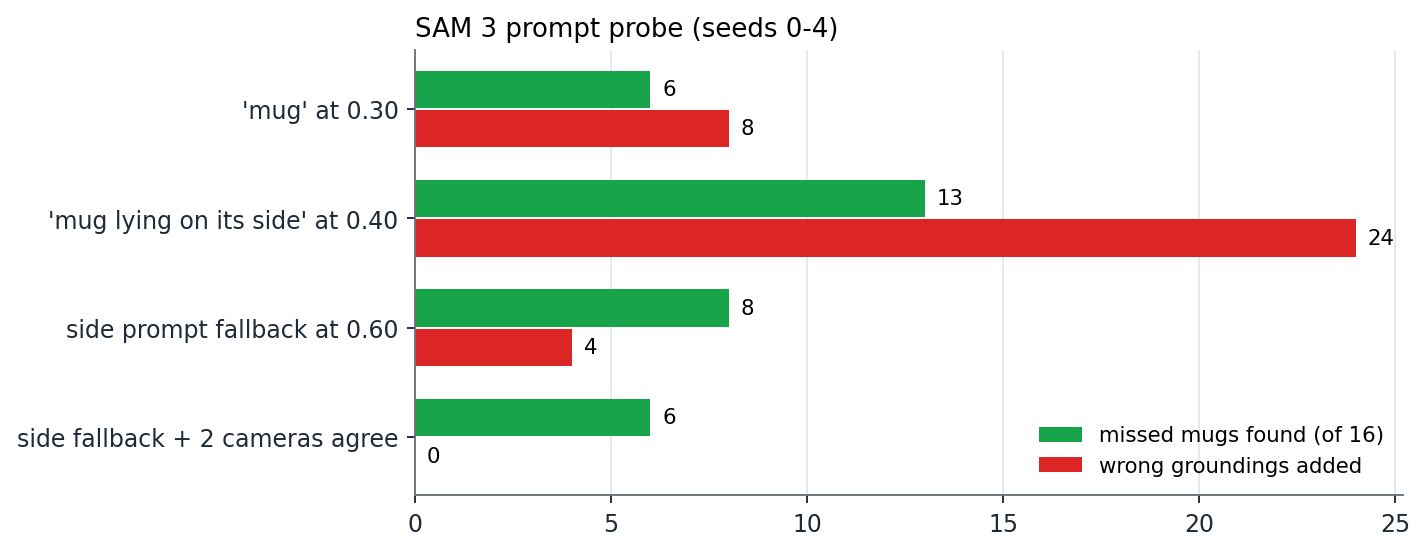
\includegraphics[width=0.78\textwidth]{figures/probe.png}
\end{center}

\begin{center}
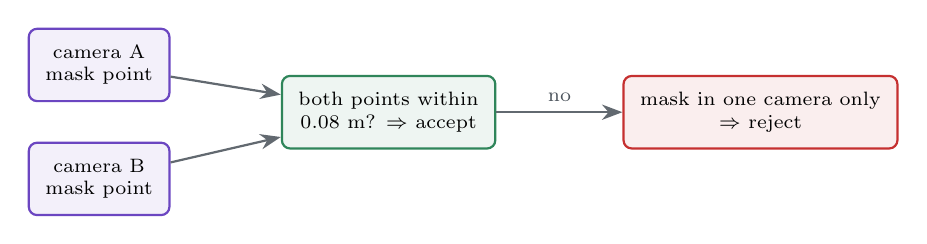
\begin{tikzpicture}
  \node[box=grape,font=\scriptsize] (c1) {camera A\\mask point};
  \node[box=grape,font=\scriptsize,below=0.5cm of c1] (c2) {camera B\\mask point};
  \node[box=leaf,font=\scriptsize,right=1.4cm of c1,yshift=-0.6cm] (ok) {both points within\\0.08 m? $\Rightarrow$ accept};
  \node[box=rose,font=\scriptsize,right=1.6cm of ok] (no) {mask in one camera only\\$\Rightarrow$ reject};
  \draw[flow] (c1) -- (ok); \draw[flow] (c2) -- (ok);
  \draw[flow] (ok) -- node[lbl,above]{no} (no);
\end{tikzpicture}
\end{center}

Every single-camera option added wrong groundings 0.2--0.6 m away (gripper, rack, other
arm). One combined rule --- fall back to ``mug lying on its side'' only when no camera finds
``mug'', and accept it only where \textbf{two cameras agree} --- found 6 of 16 with no wrong
answers. Because it was chosen by searching on these same frames, it is \textbf{frozen and
not adopted} until it passes on held-out seeds.

\subsection{Speed: render only the frames that are used}

\begin{center}
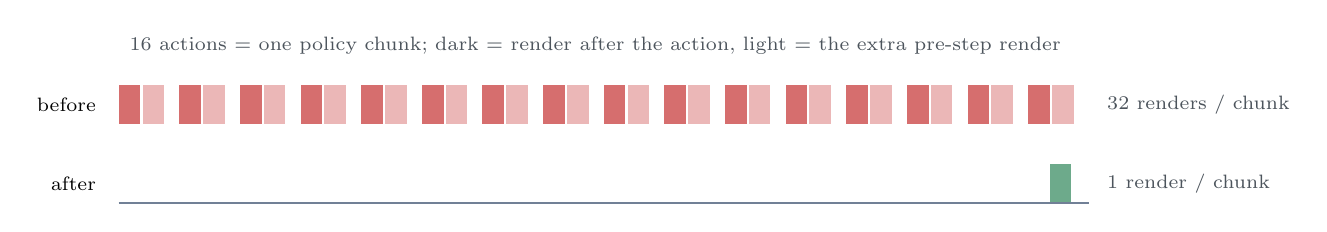
\begin{tikzpicture}[x=0.55cm]
  \node[anchor=east,font=\scriptsize] at (-0.3,1) {before};
  \foreach \i in {0,...,15} {
    \fill[rose!70] (\i*1.4,0.75) rectangle (\i*1.4+0.5,1.25);
    \fill[rose!35] (\i*1.4+0.55,0.75) rectangle (\i*1.4+1.05,1.25);
  }
  \node[anchor=east,font=\scriptsize] at (-0.3,0) {after};
  \fill[leaf!70] (21.5,-0.25) rectangle (22,0.25);
  \draw[stone] (0,-0.25) -- (22.4,-0.25);
  \node[lbl,anchor=west] at (22.6,1) {32 renders / chunk};
  \node[lbl,anchor=west] at (22.6,0) {1 render / chunk};
  \node[lbl] at (11,1.75) {16 actions = one policy chunk; dark = render after the action, light = the extra pre-step render};
\end{tikzpicture}
\end{center}

Rendering every camera with depth costs most of a simulator step (about 80\% even on a
Modal A10; about 0.8 s on a laptop RTX 2050). The capture now applies actions with the
local client's new \code{advance} method (no render) and renders only the frame the policy
needs and the frames it saves. Physics is unchanged: RoboTwin's \code{get_obs} only reads
the cameras.

\begin{center}
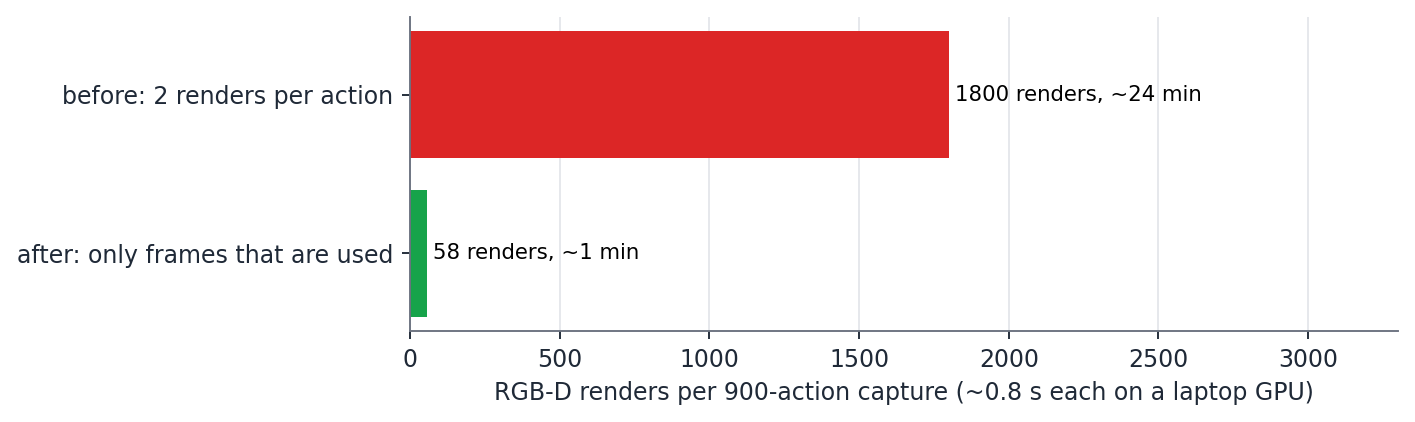
\includegraphics[width=0.78\textwidth]{figures/renders.png}
\end{center}

\textbf{Why there were two renders per step.} The base client's \code{step} calls
\code{observe()} to read the previous sequence number --- free for the HTTP client, which
returns a cached frame. The local client's \code{observe()} re-renders, because analytic
skills move the robot with \code{tick()} and a cached frame would go stale. Together:
render, discard, act, render. The new run setting \code{render_once_per_step: true} takes
those values from the client's own state instead (same observations, one render). It is
off by default so existing timings stay comparable.

\subsection{Smaller fixes along the way}

\begin{itemize}
\item \textbf{Invalid depth pixels} (non-finite or negative) now count as missing depth
  instead of rejecting the whole observation --- that had crashed a capture.
\item \textbf{Modal downloads} wait until the runs Volume shows every file.
\item \textbf{One failed seed} no longer stops a capture batch.
\item \textbf{GPU fallbacks}: \code{SIM_GPU=L4,A10G,T4} tries GPUs in order; the manifest
  records which one ran.
\item \textbf{Labels}: a mug held tilted in a gripper is not \code{toppled}.
\item \textbf{Policy-call timeout.} During the held-out capture the policy container
  vanished mid-request and Modal's \code{.remote()} waited two hours on a closed
  connection. Every policy call now gives up after 5 minutes
  (\code{POLICY_CALL_TIMEOUT_SECONDS}); the seed fails cleanly and the loop moves on.
  It does not retry: a fresh container has lost the policy's last two observations.
\end{itemize}

% ================================================================ 7b
\section{Why this matters: perception is the supervisor's eyes}

The project's supervisor is the orchestrator plus a planner (scripted or Opus), sitting
on top of the frozen Neotix policy. It decides when to let the policy act, when to stop
it, when to retry, and when it is safe to let go of the mug. Every one of those
decisions is made from predicates --- and in a real run, predicates come only from
perception. If the eyes are wrong, the supervisor is confidently wrong.

\begin{center}
\begin{tikzpicture}[node distance=1.5cm]
  \node[box=stone,minimum width=11cm,minimum height=1.0cm] (pol) {\faRobot\ \textbf{Frozen VLA policy (Neotix)}\quad\scriptsize moves both arms; never changed};
  \node[box=sun,minimum width=11cm,minimum height=1.0cm,above=of pol] (sup) {\faUserShield\ \textbf{Supervisor}\quad\scriptsize planner + orchestrator: which skill, when to stop, retry, release};
  \node[box=grape,minimum width=11cm,minimum height=1.0cm,above=of sup] (per) {\faEye\ \textbf{Perception}\quad\scriptsize cameras $\to$ SAM 3 $\to$ depth $\to$ geometry \quad\textcolor{rose}{\textbf{$\leftarrow$ this branch}}};
  \draw[flow] ([xshift=-3cm]per.south) -- node[lbl,left]{predicates:\\lifted? staged?\\safe to release?} ([xshift=-3cm]sup.north);
  \draw[flow] ([xshift=-3cm]sup.south) -- node[lbl,left]{stop / retry\\/ release} ([xshift=-3cm]pol.north);
  \draw[flow] (pol.east) -- ++(0.7,0) |- node[lbl,right,pos=0.25]{the arms move;\\cameras see it} (per.east);
\end{tikzpicture}
\end{center}

\subsection{What each fix gives the supervisor}

\begin{center}
\begin{tikzpicture}[x=5.2cm]
  \foreach \y/\q/\p/\m/\b/\a/\bt/\at/\good in {
     0/{Can I open the gripper?}/{release\_ready}/precision/0.72/1.00/{0.72}/{1.00}/{no wrong trues on seeds 0--4; one end-on case held out},
    -1.55/{Did the handoff stage work?}/{mug\_staged\_on\_table}/precision/0.62/1.00/{0.62}/{1.00}/{sees a toppled mug as a failure},
    -3.1/{Right arm has it?}/{right\_mug\_lifted}/recall/0.09/0.88/{0.09}/{0.88}/{stops stalling after a good handoff},
    -4.65/{Lifted? Stop the policy?}/{mug\_lifted}/recall/0.37/0.74/{0.37}/{0.74}/{stops the policy at the right time}} {
    \node[anchor=west,font=\small\bfseries] at (-1.02,\y+0.3) {\q};
    \node[anchor=west,font=\scriptsize\ttfamily,text=grape] at (-1.02,\y-0.15) {\p};
    \node[anchor=west,font=\scriptsize,text=stone] at (-1.02,\y-0.5) {\m};
    \fill[rose!70] (0,\y+0.12) rectangle (\b,\y+0.42); \node[anchor=west,font=\scriptsize] at (\b,\y+0.27) {\bt\ before};
    \fill[leaf!80] (0,\y-0.32) rectangle (\a,\y-0.02); \node[anchor=west,font=\scriptsize] at (\a,\y-0.17) {\at\ after};
    \node[anchor=west,font=\scriptsize,text=leaf!70!black,text width=3.3cm] at (1.42,\y+0.05) {\faCheck\ \good};
  }
  \draw[stone] (0,0.65) -- (0,-5.2);
  \node[lbl] at (0.5,-5.45) {0 \hspace{5cm} 1.0};
\end{tikzpicture}\\[2pt]
{\scriptsize\color{stone}Seeds 0--4. The first two compare the baseline with the toppled fix; the last two compare without and with the perception camera, all fixes on.}
\end{center}

\subsection{Idea 1: a supervisor must intervene safely}

\begin{center}
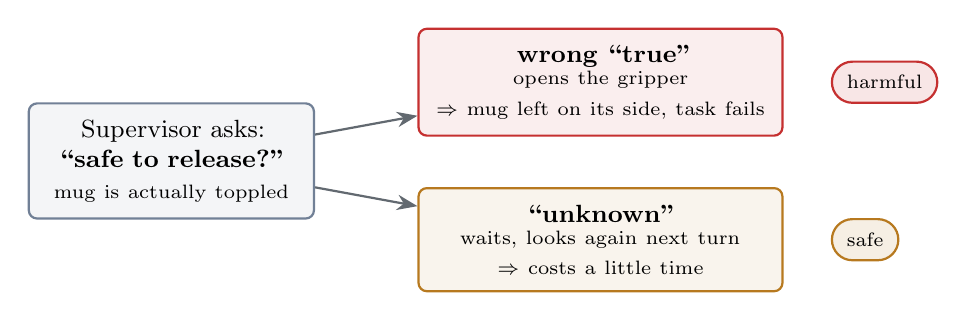
\begin{tikzpicture}[node distance=0.5cm and 0.8cm]
  \node[box=stone,text width=3.2cm] (q) {Supervisor asks:\\\textbf{``safe to release?''}\\\scriptsize mug is actually toppled};
  \node[box=rose,text width=4.2cm,right=1.3cm of q,yshift=1.0cm] (wt) {\textbf{wrong ``true''}\\\scriptsize opens the gripper\\$\Rightarrow$ mug left on its side, task fails};
  \node[box=sun,text width=4.2cm,right=1.3cm of q,yshift=-1.0cm] (wu) {\textbf{``unknown''}\\\scriptsize waits, looks again next turn\\$\Rightarrow$ costs a little time};
  \node[pill=rose,right=0.6cm of wt,font=\scriptsize] {harmful};
  \node[pill=sun,right=0.6cm of wu,font=\scriptsize] {safe};
  \draw[flow] (q) -- (wt); \draw[flow] (q) -- (wu);
\end{tikzpicture}
\end{center}

A supervisor is only worth having if it does not make the policy worse. That is why every
fix aims to keep \code{release_ready}, \code{mug_staged_on_table} and \code{right_mug_lifted}
at \textbf{precision 1.00}: the supervisor should never act on a false fact; lower recall
only makes it more patient. On the development seeds all three reached 1.00. On the
held-out seeds \code{right_mug_lifted} stayed at 1.00, but a toppled mug seen end-on
by the head camera gave 25 wrong \code{release_ready} answers (Section~7.2) --- exactly
the kind of error the held-out test exists to catch.

\subsection{Idea 2: a supervisor must notice failure}

The policy topples, drops or misses the mug and does not notice. Before this branch, the
supervisor did not notice either.

\begin{center}
\begin{tikzpicture}[x=1cm,y=1cm]
  \node[font=\small\bfseries,anchor=west] at (-0.2,1.45) {Before};
  \node[box=stone,font=\scriptsize] (a1) at (1.3,0.55) {policy\\topples mug};
  \node[box=rose,font=\scriptsize] (a2) at (4.4,0.55) {``staged on table''\\\faCheck\ (wrong)};
  \node[box=rose,font=\scriptsize] (a3) at (7.6,0.55) {release, start\\right-arm grasp};
  \node[box=rose,font=\scriptsize] (a4) at (10.7,0.55) {fails later,\\cause unclear};
  \draw[flow] (a1)--(a2); \draw[flow] (a2)--(a3); \draw[flow] (a3)--(a4);
  \node[font=\small\bfseries,anchor=west] at (-0.2,-0.55) {After};
  \node[box=stone,font=\scriptsize] (b1) at (1.3,-1.45) {policy\\topples mug};
  \node[box=leaf,font=\scriptsize] (b2) at (4.4,-1.45) {``surface faces up''\\\faTimes\ not staged};
  \node[box=leaf,font=\scriptsize] (b3) at (7.6,-1.45) {keep holding,\\retry or recover};
  \node[box=leaf,font=\scriptsize] (b4) at (10.7,-1.45) {failure is visible\\and named};
  \draw[flow] (b1)--(b2); \draw[flow] (b2)--(b3); \draw[flow] (b3)--(b4);
\end{tikzpicture}
\end{center}

The settle rule does the same for a mug that is still moving: ``touching the table'' in
one frame is no longer enough to call it placed.

\subsection{Idea 3: no cheating --- the supervisor must work without the answer key}

\begin{center}
\begin{tikzpicture}
  \node[box=rose,text width=4.6cm] (o) {\faKey\ \textbf{Oracle supervisor}\\\scriptsize reads exact mug pose and contacts from the simulator};
  \node[box=grape,text width=4.6cm,below=0.6cm of o] (c) {\faCamera\ \textbf{Camera supervisor}\\\scriptsize sees only RGB-D images, like a real robot};
  \node[box=stone,text width=4.4cm,right=1.6cm of o] (os) {works in simulation only\\\scriptsize proves the planner logic, not the system};
  \node[box=leaf,text width=4.4cm,right=1.6cm of c] (cs) {could run on a real robot\\\scriptsize this branch measures what it costs};
  \draw[dflow] (o) -- (os); \draw[flow] (c) -- (cs);
\end{tikzpicture}
\end{center}

Until now the supervisor could be shown working only with the oracle. This branch shows
how well it can run on camera evidence alone, and puts a number on the gap. That is what
makes ``an agent-aware supervisor improves a frozen VLA'' a credible claim.

\subsection{Telling a perception error from a supervisor error}

\begin{center}
\begin{tikzpicture}[node distance=0.6cm and 1.0cm]
  \node[box=stone] (f) {\faTimesCircle\ supervised episode failed};
  \node[box=sky,below=of f,text width=5.4cm] (q) {look up the predicates the supervisor used\\in the evaluator (\code{frames.jsonl}): were they right?};
  \node[box=grape,below left=0.8cm and -1.2cm of q,text width=4.2cm] (p) {\textbf{a fact was wrong}\\\scriptsize $\Rightarrow$ perception problem: fix the provider, re-score offline};
  \node[box=sun,below right=0.8cm and -1.2cm of q,text width=4.2cm] (s) {\textbf{facts were right}\\\scriptsize $\Rightarrow$ supervisor logic problem: fix the planner or skill};
  \draw[flow] (f) -- (q); \draw[flow] (q) -- node[lbl,left]{no} (p); \draw[flow] (q) -- node[lbl,right]{yes} (s);
\end{tikzpicture}
\end{center}

\subsection{What the supervisor still cannot see well}

\begin{center}
\begin{tikzpicture}[node distance=0.4cm]
  \node[box=sun,text width=4.3cm,minimum height=2.2cm] (m1) {\faEyeSlash\ \textbf{Sideways mugs at the rack}\\\scriptsize often ``unknown'': the supervisor waits or stops instead of guessing --- safe, but can cost success};
  \node[box=sun,text width=4.3cm,minimum height=2.2cm,right=of m1] (m2) {\faBullseye\ \textbf{Rack predicates}\\\scriptsize \code{mug_near_rack}, \code{rack_seat_aligned} are not yet scored by this evaluator --- next for the HANG phase};
  \node[box=sun,text width=4.3cm,minimum height=2.2cm,right=of m2] (m3) {\faClock\ \textbf{Cost per check}\\\scriptsize every check is a SAM 3 call: perception runs at turn boundaries, and render speed matters for live runs};
\end{tikzpicture}
\end{center}

\begin{keyidea}
Perception does not make the supervisor smarter; it makes the supervisor's facts
\emph{trustworthy enough that its interventions help instead of hurt}. The held-out seeds
5--9 test whether that still holds on episodes no rule was tuned on.
\end{keyidea}

% ================================================================ 8
\section{The commands, in order, and why}

\begin{center}
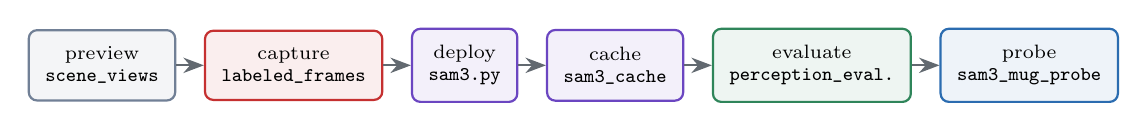
\begin{tikzpicture}[node distance=0.35cm]
  \node[box=stone,font=\scriptsize] (v) {preview\\\code{scene_views}};
  \node[box=rose,font=\scriptsize,right=of v] (c) {capture\\\code{labeled_frames}};
  \node[box=grape,font=\scriptsize,right=of c] (d) {deploy\\\code{sam3.py}};
  \node[box=grape,font=\scriptsize,right=of d] (s) {cache\\\code{sam3_cache}};
  \node[box=leaf,font=\scriptsize,right=of s] (e) {evaluate\\\code{perception_eval.}};
  \node[box=sky,font=\scriptsize,right=of e] (p) {probe\\\code{sam3_mug_probe}};
  \draw[flow] (v)--(c); \draw[flow] (c)--(d); \draw[flow] (d)--(s); \draw[flow] (s)--(e); \draw[flow] (e)--(p);
\end{tikzpicture}
\end{center}

\begin{careful}
\textbf{One GPU job at a time.} The deployed policy keeps a single observation history,
so two captures or episodes at once would mix their histories.
\end{careful}

\subsubsection*{Preview a camera (local, no policy)}
\begin{cmd}
python -m development.capture.scene\_views -{}-seed 3 \textbackslash\\
\ \ -{}-output data/scenes/seed\_3\_cam -{}-perception-camera default
\end{cmd}
\emph{Why:} see what each camera covers before spending GPU time.

\subsubsection*{Capture labelled frames (seeds)}
On Modal (fast, uses Modal units for the simulator GPU and the policy):
\begin{cmd}
SIM\_GPU=L4,A10G,T4 modal run modal\_apps/simulator.py::frames \textbackslash\\
\ \ -{}-seeds 0,1,2,3,4 -{}-perception-camera default \textbackslash\\
\ \ -{}-output-root data/perception/frames\_cam
\end{cmd}
Locally (now a few minutes per seed; only the policy uses Modal):
\begin{cmd}
for s in 6 7 8 9; do\\
\ \ conda run -n robotwin python -m development.capture.labeled\_frames -{}-seed \$s \textbackslash\\
\ \ \ \ -{}-output data/perception/frames\_holdout/seed\_\$s -{}-perception-camera default\\
done
\end{cmd}
\emph{Why:} a seed fixes the starting scene; the policy then runs up to 900 actions, and a
frame plus a label is saved every 16 actions ($\approx$58 frames, $\approx$45 MB per seed).

\subsubsection*{Deploy SAM 3 and cache its answers}
\begin{cmd}
modal deploy modal\_apps/sam3.py\\
python -m development.replays.sam3\_cache -{}-frames data/perception/frames\_cam/seed\_0
\end{cmd}
\emph{Why:} pay for SAM 3 once per frame and camera; every later evaluation is free.

\subsubsection*{Evaluate (CPU, seconds)}
\begin{cmd}
python -m development.replays.perception\_evaluation \textbackslash\\
\ \ -{}-frames data/perception/frames\_cam/seed\_0 ... -{}-frames .../seed\_4 \textbackslash\\
\ \ -{}-output data/perception/reports/with\_camera\\[3pt]
\# same frames as if the new camera did not exist:\\
... -{}-output data/perception/reports/without\_camera -{}-ignore-camera perception\_camera
\end{cmd}
\emph{Why:} writes \code{summary.md} (detection by state, precision/recall per predicate)
and \code{frames.jsonl} (every frame's answer and reason).

\subsubsection*{Probe SAM 3 prompts}
\begin{cmd}
python -m development.replays.sam3\_mug\_probe -{}-query -{}-frames .../seed\_0 ...\ \ \# GPU\\
python -m development.replays.sam3\_mug\_probe -{}-frames .../seed\_0 ... \textbackslash\\
\ \ -{}-runtime-report data/perception/reports/with\_camera/frames.jsonl\ \ \# CPU
\end{cmd}
\emph{Why:} test new prompts or thresholds on exactly the frames the runtime misses,
without changing the runtime.

\subsubsection*{Held-out seeds (5--9): capture, cache, evaluate, probe}
\begin{cmd}
for s in 5 6 7 8 9; do\\
\ \ conda run -n robotwin python -m development.capture.labeled\_frames -{}-seed \$s \textbackslash\\
\ \ \ \ -{}-output data/perception/frames\_holdout/seed\_\$s -{}-perception-camera default \textbar\textbar\ echo "seed \$s failed"\\
done\\
\# then the same loop with: python -m development.replays.sam3\_cache -{}-frames .../seed\_\$s\\
python -m development.replays.perception\_evaluation -{}-frames .../seed\_5 ... -{}-frames .../seed\_9 \textbackslash\\
\ \ -{}-output data/perception/reports/holdout\_with\_camera
\end{cmd}
\emph{Why:} every threshold was chosen on seeds 0--4; seeds 5--9 are scored with the rules
frozen. If a seed fails or hangs, move its folder aside
(\code{mv .../seed_6 .../partial_seed_6}) before rerunning it: the capture never writes
into an existing folder. The cache step skips seeds that already have a cache.

\subsubsection*{Tests}
\begin{cmd}
conda run -n robotwin python -m pytest -q tests
\end{cmd}

% ================================================================ 9
\section{Where we are, and what is next}

\begin{center}
\small
\begin{tabular}{@{}lcccc@{}}
\toprule
\textbf{Predicate} & \textbf{Baseline} & \textbf{Fixes, no camera} & \textbf{Fixes + camera} & \textbf{Held out + camera} \\
 & \scriptsize seeds 0--4 & \scriptsize seeds 0--4 & \scriptsize seeds 0--4 & \scriptsize seeds 5--9 \\
\midrule
\code{mug_lifted} & 1.00 / 0.71 & 1.00 / 0.37 & 1.00 / 0.74 & 1.00 / 0.81 \\
\code{release_ready} & \textcolor{rose}{0.72} / 0.79 & 1.00 / 0.63 & 1.00 / 0.81 & \textcolor{rose}{0.81} / 0.83 \\
\code{mug_staged_on_table} & \textcolor{rose}{0.62} / 0.70 & 1.00 / 0.47 & 1.00 / 0.82 & \textcolor{rose}{0.75} / 0.81 \\
\code{right_mug_lifted} & 1.00 / 0.09 & 1.00 / 0.52 & 1.00 / 0.88 & 1.00 / 0.72 \\
\bottomrule
\end{tabular}\\[3pt]
{\scriptsize\color{stone}Each cell is precision / recall. Baseline: 236 frames, first capture, head + wrists. Middle two: 216 frames of
a second capture, scored without and with the new camera. Held out: 267 frames of seeds 5--9, rules frozen. Different episodes in
each capture, so compare columns of the same capture.}
\end{center}

\begin{center}
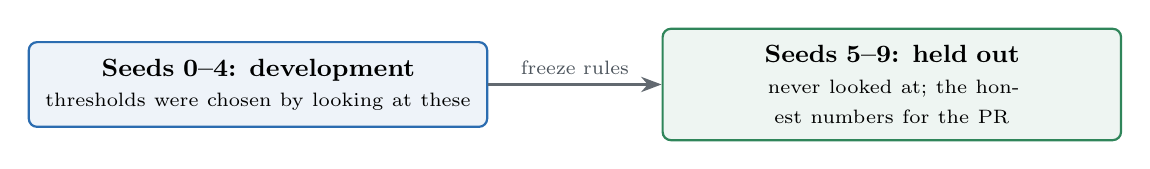
\begin{tikzpicture}
  \node[box=sky,text width=5.4cm] (dev) {\textbf{Seeds 0--4: development}\\\scriptsize thresholds were chosen by looking at these};
  \node[box=leaf,text width=5.4cm,right=2.2cm of dev] (ho) {\textbf{Seeds 5--9: held out}\\\scriptsize never looked at; the honest numbers for the PR};
  \draw[flow] (dev) -- node[lbl,above]{freeze rules} (ho);
\end{tikzpicture}
\end{center}

\begin{center}
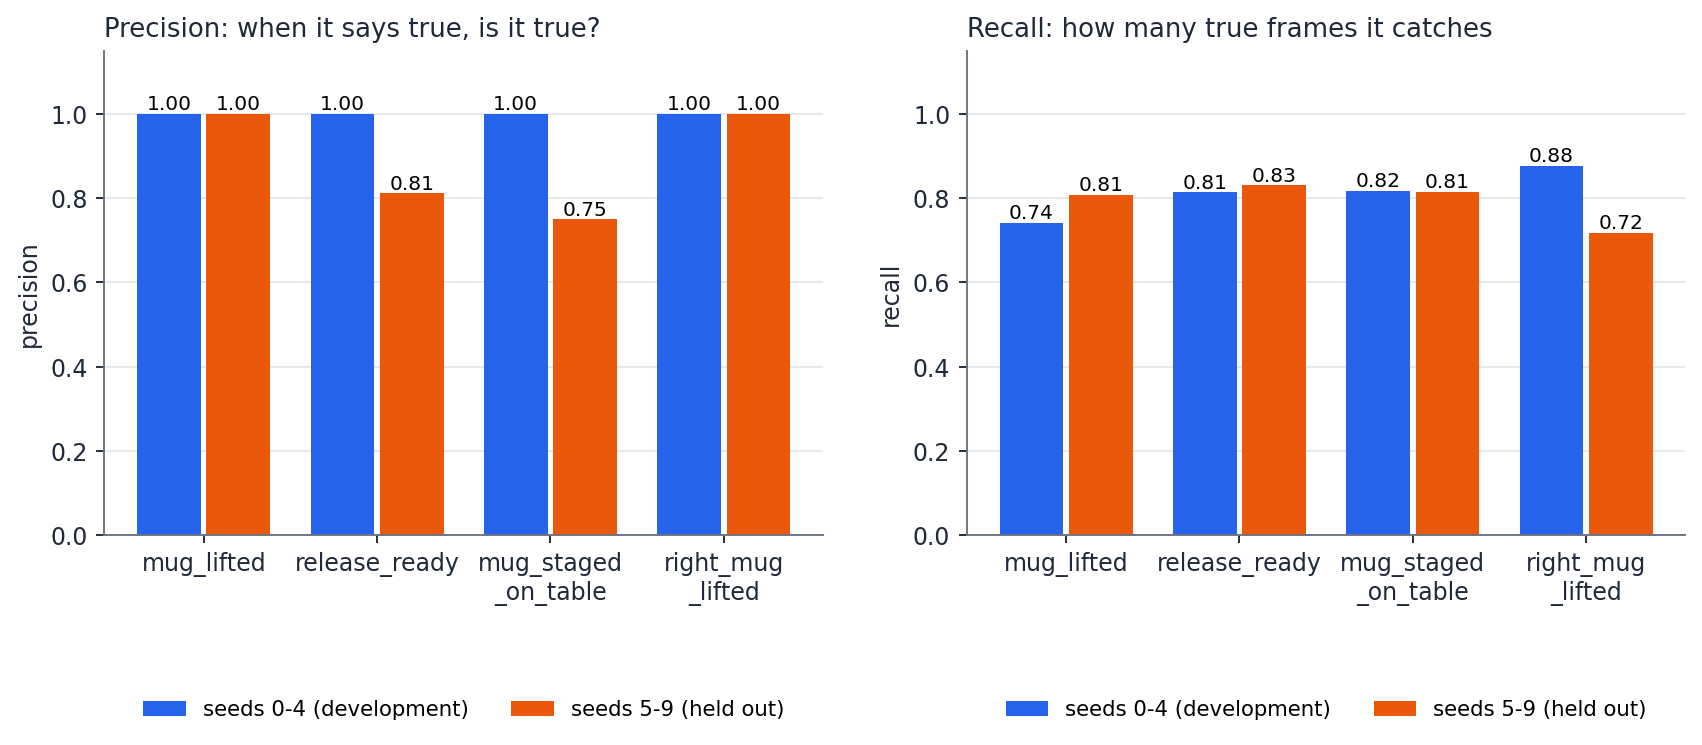
\includegraphics[width=\textwidth]{figures/holdout_results.png}\\
{\small\color{stone}With the perception camera. All 25 held-out wrong trues come from the one end-on toppled mug in seed 6;
without that episode both predicates keep precision 1.00 (recall 0.83 and 0.81).}
\end{center}

\textbf{What the held-out seeds confirmed:} \code{mug_lifted} and \code{right_mug_lifted}
keep precision 1.00 (the 0.24 m association held; right-arm recall fell to 0.72, still
far above the 0.09 baseline); the settle rule caused no wrong trues; the perception
camera again lifts every recall (held-right detection 0.32 $\to$ 0.68).
\textbf{What it broke:} the toppled test, for a mug lying with its base towards the head camera.

\begin{enumerate}
\item[\faCheck] Captured seeds 5--9 with the camera, cached SAM 3, evaluated with every rule frozen.
\item Fix the end-on toppled case \emph{using development seeds only}, then confirm it on
  fresh seeds (10--14): seeds 5--9 have now been looked at, so tuning on them would no
  longer be an honest test.
\item Probe seeds 5--9 (running): adopt the frozen two-camera rule only if it still finds
  misses with zero wrong groundings.
\item Decide whether the perception camera and \code{render_once_per_step} are on by
  default, using measured render cost.
\item One PR from \code{perception/grounding-evaluation} with the before/after tables.
\end{enumerate}

% ================================================================ 10
\section*{Glossary}
\addcontentsline{toc}{section}{Glossary}
\small
\begin{tabularx}{\textwidth}{@{}lX@{}}
\toprule
Predicate & a named true/false/unknown fact the planner and skills rely on \\
Provider & the object that answers predicates (camera or oracle) \\
Planner & chooses one skill per turn from images and predicates \\
Skill & a bounded robot action (\code{vla_act}, \code{move_to}, \code{set_gripper}, \dots) \\
Oracle & answers from exact simulator state; development only \\
SAM 3 & segmentation model: paints the pixels of a named object \\
Mask & the set of pixels SAM 3 assigned to an object \\
Grounding & turning a mask plus depth into a 3D position \\
Latch & once true, stays true for the episode \\
Precision / recall & is ``true'' right? / how many true frames were caught? \\
Seed & fixes the starting scene; the policy still varies \\
Held-out & frames never used to choose a threshold \\
TCP & tool centre point: the arm's measured end-effector frame \\
\bottomrule
\end{tabularx}

\normalsize
\appendix
\clearpage
\section{Plan: recovering a toppled mug}

\begin{keyidea}
Goal: when the policy topples the mug, the supervisor sends bounded skill commands that
pick the mug up, stand it upright at the place where the left hand normally sets it down,
and then continue the normal handoff. \textbf{This is a plan; none of it is implemented
yet.}
\end{keyidea}

\subsection{The recovery as a chain of skills and checks}

\begin{center}
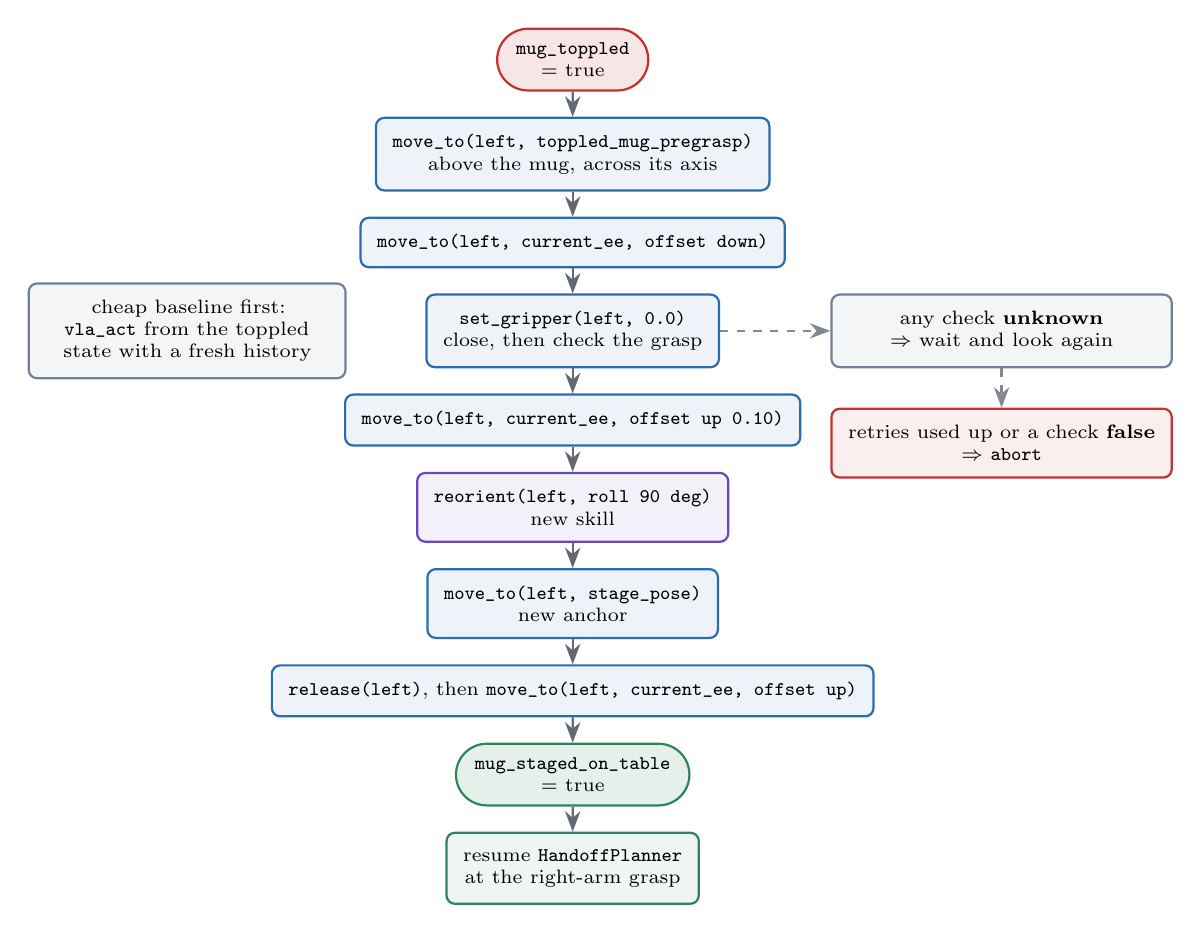
\begin{tikzpicture}[node distance=0.32cm]
  \node[pill=rose,font=\scriptsize] (t) {\code{mug_toppled}\\= true};
  \node[box=sky,font=\scriptsize,below=of t] (s1) {\code{move_to(left, toppled_mug_pregrasp)}\\\scriptsize above the mug, across its axis};
  \node[box=sky,font=\scriptsize,below=of s1] (s2) {\code{move_to(left, current_ee, offset down)}};
  \node[box=sky,font=\scriptsize,below=of s2] (s3) {\code{set_gripper(left, 0.0)}\\\scriptsize close, then check the grasp};
  \node[box=sky,font=\scriptsize,below=of s3] (s4) {\code{move_to(left, current_ee, offset up 0.10)}};
  \node[box=grape,font=\scriptsize,below=of s4] (s5) {\textbf{\code{reorient(left, roll 90 deg)}}\\\scriptsize new skill};
  \node[box=sky,font=\scriptsize,below=of s5] (s6) {\code{move_to(left, stage_pose)}\\\scriptsize new anchor};
  \node[box=sky,font=\scriptsize,below=of s6] (s7) {\code{release(left)}, then \code{move_to(left, current_ee, offset up)}};
  \node[pill=leaf,font=\scriptsize,below=of s7] (g) {\code{mug_staged_on_table}\\= true};
  \node[box=leaf,font=\scriptsize,below=of g] (r) {resume \code{HandoffPlanner}\\at the right-arm grasp};
  \foreach \a/\b in {t/s1,s1/s2,s2/s3,s3/s4,s4/s5,s5/s6,s6/s7,s7/g,g/r} \draw[flow] (\a) -- (\b);
  \node[box=stone,font=\scriptsize,text width=3.9cm,right=1.4cm of s3] (u) {any check \textbf{unknown}\\$\Rightarrow$ wait and look again};
  \node[box=rose,font=\scriptsize,text width=3.9cm,below=0.5cm of u] (a) {retries used up or a check \textbf{false}\\$\Rightarrow$ \code{abort}};
  \draw[dflow] (s3.east) -- (u.west); \draw[dflow] (u) -- (a);
  \node[box=stone,font=\scriptsize,text width=3.6cm,left=1.0cm of s3] (b) {cheap baseline first:\\\code{vla_act} from the toppled state with a fresh history};
\end{tikzpicture}
\end{center}

\subsection{What exists and what is missing}

\begin{center}
\begin{tikzpicture}
  \node[box=leaf,font=\scriptsize,text width=7.0cm,align=left,anchor=north] (e) at (0,0) {
   \textbullet\ skills: \code{move_to} (named target + offset $\le$ 20 cm), \code{rotate_wrist} (yaw $\pm$30$^\circ$),
   \code{set_gripper}, \code{release}, \code{vla_act}, \code{abort}\\
   \textbullet\ anchors: \code{current_ee}, \code{mug_pregrasp}, \code{rack_approach}, \code{table_approach}, \code{rack_seat}\\
   \textbullet\ \code{HandoffPlanner} phases and predicate gates\\
   \textbullet\ CuRobo planning to any full pose (\code{plan})\\
   \textbullet\ the surface-normal toppled evidence (as a reason)\\
   \textbullet\ checkpoint bank and \code{manual_skill.py} for rehearsing skills};
  \node[box=rose,font=\scriptsize,text width=7.0cm,align=left,anchor=north] (m) at (8.3,0) {
   \textbf{1.} \code{mug_toppled} predicate (needs the end-on fix first)\\
   \textbf{2.} \code{toppled_mug_pregrasp} anchor: axis direction and grasp from depth\\
   \textbf{3.} \code{stage_pose} anchor: the handover place, defined publicly\\
   \textbf{4.} \code{reorient} skill: about 90$^\circ$ roll through CuRobo\\
   \textbf{5.} planner recovery phase (+ Opus schema, new prompt version)\\
   \textbf{6.} toppled checkpoints and a recovery evaluation};
  \node[font=\small\bfseries,text=leaf,above=0.15cm of e] {\faCheck\ Already in the code};
  \node[font=\small\bfseries,text=rose,above=0.15cm of m] {\faPlus\ To build};
\end{tikzpicture}
\end{center}

\subsection{The perception pieces}

\textbf{1. A \code{mug_toppled} predicate.} Today ``toppled'' only blocks
\code{release_ready}. Recovery needs a fact the planner can branch on: true when the
mug is grounded from the head or perception camera, touches the table and its surface
faces up. It inherits the end-on blind spot from seed 6 (it would say false there), so
that fix comes first --- designed on seeds 0--4, confirmed on fresh seeds 10--14.

\textbf{2. Where it lies and which way.} A pick-up needs the mug's axis and its open end,
not just its centre.

\begin{center}
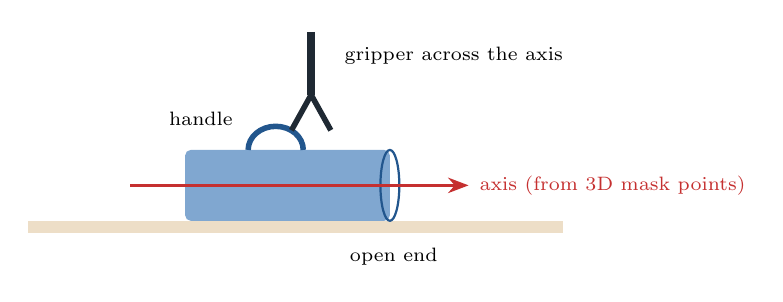
\begin{tikzpicture}
  \fill[sun!25] (-3.4,-0.15) rectangle (3.4,0);
  \fill[sky!60,rounded corners=2pt] (-1.4,0) rectangle (1.2,0.9);
  \draw[sky!80!black,line width=2pt] (-0.6,0.9) arc (180:0:0.35 and 0.3);
  \draw[sky!80!black,thick] (1.2,0.45) ellipse (0.12 and 0.45);
  \draw[->,very thick,rose] (-2.1,0.45) -- (2.2,0.45) node[right,font=\scriptsize]{axis (from 3D mask points)};
  \node[font=\scriptsize] at (1.25,-0.45) {open end};
  \node[font=\scriptsize] at (-1.2,1.3) {handle};
  \draw[ink,line width=3pt] (0.2,2.4) -- (0.2,1.6);
  \draw[ink,line width=2pt] (0.2,1.6) -- (-0.05,1.15) (0.2,1.6) -- (0.45,1.15);
  \node[font=\scriptsize,anchor=west] at (0.5,2.1) {gripper across the axis};
\end{tikzpicture}
\end{center}

The long direction of the mask's 3D points gives the axis (it lies horizontal); the end
whose depth shows a hollow gives the opening. Trusted perception code turns that into a
fresh \code{toppled_mug_pregrasp} anchor each observation --- never simulator poses.

\textbf{3. A public ``handover place''.} The left hand sets the mug where the
\emph{policy} chooses, near RoboTwin's \code{middle_pos} --- simulator truth, so not
usable at runtime. Define \code{stage_pose} as a fixed pose in the table frame, taught once
and stored in config (like a taught position on a real robot), or as the median position
where perception saw the mug when \code{mug_staged_on_table} first became true in successful
development runs, frozen into config.

\subsection{The motion piece: standing it up}

\begin{center}
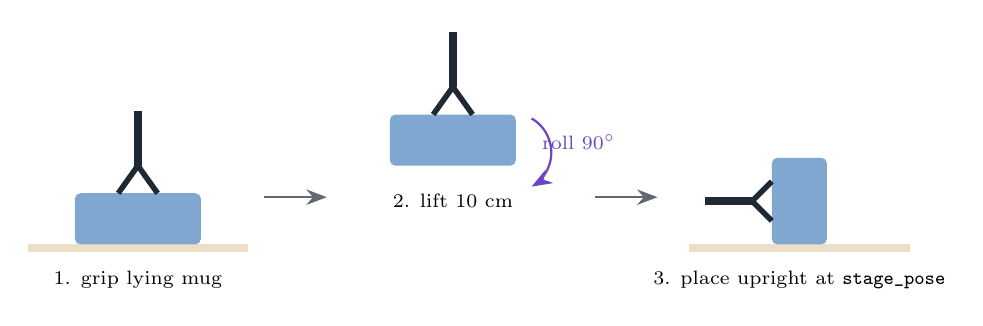
\begin{tikzpicture}
  \begin{scope}
    \fill[sun!25] (-1.4,-0.1) rectangle (1.4,0);
    \fill[sky!60,rounded corners=2pt] (-0.8,0) rectangle (0.8,0.65);
    \draw[ink,line width=3pt] (0,1.7) -- (0,1.0); \draw[ink,line width=2pt] (0,1.0) -- (-0.25,0.65) (0,1.0) -- (0.25,0.65);
    \node[font=\scriptsize] at (0,-0.45) {1. grip lying mug};
  \end{scope}
  \draw[flow] (1.6,0.6) -- (2.4,0.6);
  \begin{scope}[xshift=4cm]
    \fill[sky!60,rounded corners=2pt] (-0.8,1.0) rectangle (0.8,1.65);
    \draw[ink,line width=3pt] (0,2.7) -- (0,2.0); \draw[ink,line width=2pt] (0,2.0) -- (-0.25,1.65) (0,2.0) -- (0.25,1.65);
    \draw[->,thick,grape] (1.0,1.6) arc (60:-60:0.5); \node[font=\scriptsize,text=grape] at (1.6,1.3) {roll 90$^\circ$};
    \node[font=\scriptsize] at (0,0.55) {2. lift 10 cm};
  \end{scope}
  \draw[flow] (5.8,0.6) -- (6.6,0.6);
  \begin{scope}[xshift=8.4cm]
    \fill[sun!25] (-1.4,-0.1) rectangle (1.4,0);
    \fill[sky!60,rounded corners=2pt] (-0.35,0) rectangle (0.35,1.1);
    \draw[ink,line width=3pt] (-1.2,0.55) -- (-0.6,0.55); \draw[ink,line width=2pt] (-0.6,0.55) -- (-0.35,0.8) (-0.6,0.55) -- (-0.35,0.3);
    \node[font=\scriptsize] at (0,-0.45) {3. place upright at \code{stage_pose}};
  \end{scope}
\end{tikzpicture}
\end{center}

\code{rotate_wrist} only turns $\pm$30$^\circ$ about the vertical. Standing a mug up needs
about 90$^\circ$ about a horizontal axis: a new bounded \code{reorient} skill (axis and angle,
angle limited to about $\pm$90$^\circ$, planned with CuRobo to a full pose), or \code{move_to}
accepting a named target orientation such as ``upright at \code{stage_pose}''.

\begin{careful}
\textbf{Check feasibility first.} The Aloha arms have 6 joints, so a 90$^\circ$ roll above the
table may not be reachable everywhere. The gripper opening against the mug's $\approx$8 cm
diameter decides whether the body can be gripped or the rim at the open end must be pinched
(as a person would). If the arm cannot do this with perfect positions, the perception work for
it is not worth building yet.
\end{careful}

\subsection{How to develop it safely}

\begin{center}
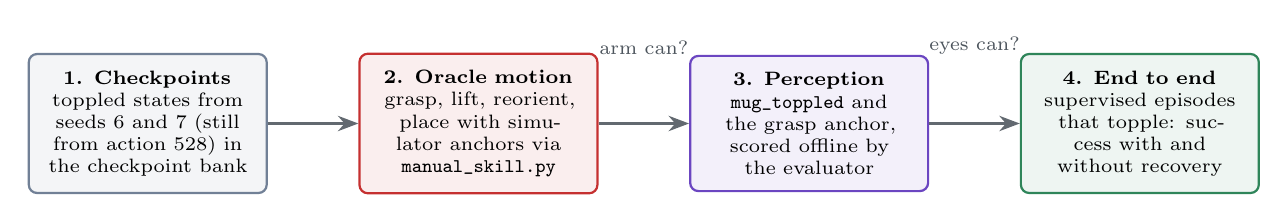
\begin{tikzpicture}[node distance=1.15cm]
  \node[box=stone,text width=2.6cm,font=\scriptsize] (c) {\textbf{1. Checkpoints}\\toppled states from seeds 6 and 7 (still from action 528) in the checkpoint bank};
  \node[box=rose,text width=2.6cm,font=\scriptsize,right=of c] (o) {\textbf{2. Oracle motion}\\grasp, lift, reorient, place with simulator anchors via \code{manual_skill.py}};
  \node[box=grape,text width=2.6cm,font=\scriptsize,right=of o] (p) {\textbf{3. Perception}\\\code{mug_toppled} and the grasp anchor, scored offline by the evaluator};
  \node[box=leaf,text width=2.6cm,font=\scriptsize,right=of p] (e) {\textbf{4. End to end}\\supervised episodes that topple: success with and without recovery};
  \draw[flow] (c) -- (o); \draw[flow] (o) -- node[lbl,above=0.75cm]{arm can?} (p); \draw[flow] (p) -- node[lbl,above=0.75cm]{eyes can?} (e);
\end{tikzpicture}
\end{center}

Step 2 separates ``can the arm do it?'' from step 3's ``can perception see it?''. Each new
predicate is scored for precision before the planner may act on it, as for every predicate in
this branch.

\subsection{Effort and risk}

\begin{center}
\small
\begin{tabularx}{\textwidth}{@{}Xll@{}}
\toprule
\textbf{Piece} & \textbf{Effort} & \textbf{Risk} \\
\midrule
\code{mug_toppled} predicate & small, after the end-on fix & medium (end-on views) \\
Axis and grasp anchor from depth & medium & medium \\
\code{stage_pose} anchor from config & small & low \\
\code{reorient} skill with CuRobo & medium--large & \textcolor{rose}{\textbf{high}} (reachability, gripper fit) \\
Planner phase and Opus schema & medium & low \\
\bottomrule
\end{tabularx}
\end{center}

\textbf{Start with steps 1 and 2} --- checkpoints and oracle motion --- before any perception code.

\end{document}
